% !TeX spellcheck = it_IT
\title{GPU Computing}
\author{Massimo Perego}
\date{}

\documentclass[11pt]{article}
\usepackage{graphicx} 
\usepackage{amsmath}
\usepackage{amssymb}
\usepackage{amsfonts}
\usepackage{graphicx}
\usepackage[hidelinks]{hyperref}
\usepackage[autostyle, english = american]{csquotes}
\usepackage[parfill]{parskip}
\MakeOuterQuote{"}
\usepackage{xcolor}
\definecolor{bg}{rgb}{0.95,0.95,0.95}
\definecolor{g}{rgb}{0,0.5,0.1}
\usepackage{minted}
\setminted[c]{linenos, bgcolor=bg}
\setminted[python]{linenos, bgcolor=bg}
\setminted[java]{bgcolor=bg}
\usepackage{tikz}
\usetikzlibrary{trees, arrows.meta, positioning, calc}

\tikzstyle{block} = [draw, rectangle, minimum height=2em, minimum width=3em]

\renewcommand{\contentsname}{Indice}

\newcommand{\np}{\mathcal{NP}}

\begin{document}
	\maketitle
	\tableofcontents
	\newpage	
	
	% !TeX spellcheck = it_IT
\section{Introduzione all'High Performance Computing HPC}

L'uso delle GPU permette di incrementare significativamente le performance, per avere speed-up anche nell'ordine delle migliaia, per problemi altamente parallelizzabili. Si parlerà di paradigma \textbf{GP-GPU} (\textbf{General Purpose - GPU}).

Esistono molti sistemi che si basano su operazioni semplici ma ripetute numerose volte. Esempio: il prodotto matriciale è il prodotto vettore-vettore ripetuto. Questi sistemi sono facilmente parallelizzabili (se non ci sono interdipendenze tra i risultati).

\paragraph{Parallelismo:} Vogliamo accelerare il tempo, il parallelismo è la capacità di eseguire parti di un calcolo in modo concorrente. Esistono problemi che sarebbero impensabili senza l'accelerazione permessa dal parallelismo. Permette di risolvere problemi più grandi nello stesso tempo, o problemi di dimensione fissa in tempo più breve.

Il parallelismo sarà gestito a livello di \textbf{thread}: unità di esecuzione costituita da una sequenza di istruzioni e gestita dal sistema operativo o da un sistema di runtime.

\paragraph{Paradigma GP-GPU:} Fa riferimento all'uso di GPU (Graphics Processing Unit) per eseguire computazioni di carattere generale, di qualsiasi tipo. Implica l'uso di CPU e GPU in maniera congiunta, la computazione parte comunque dalla CPU (chiamata \textbf{host}) la quale effettuerà richieste alla GPU (chiamata \textbf{device}), quest'ultima diventa un coprocessore. Viene separata la parte sequenziale dell'applicazione e di controllo, che va sulla CPU, dalla parte a maggior intensità computazionale, lasciata alla GPU.

La GPU non è una piattaforma stand-alone, ma è un coprocessore che opera congiuntamente alla CPU, comunicando tramite bus PCI-Express. Sono necessari trasferimenti e la CPU orchestra la "sincronizzazione".
\begin{center}
	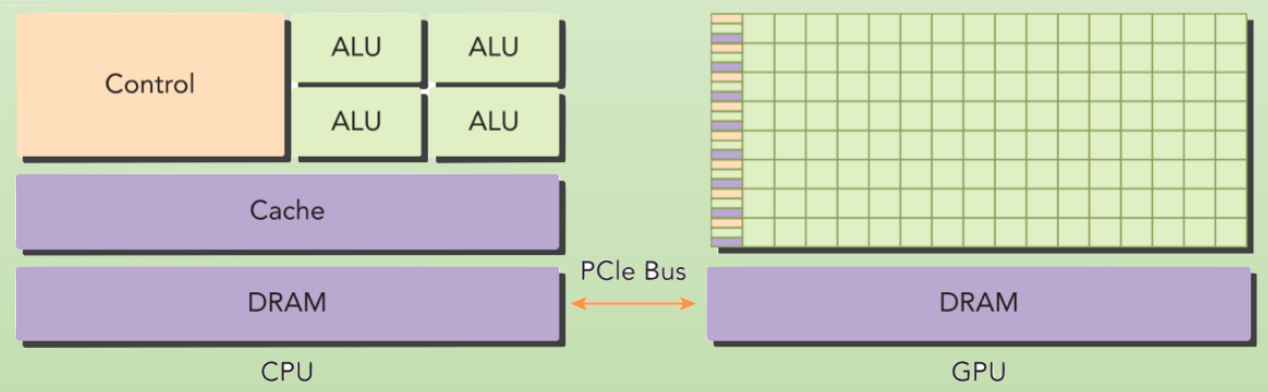
\includegraphics[width=0.95\linewidth]{img/intro/gpgpu1}
\end{center}

L'uso, dal punto di vista dell'utente, di un sistema con GPU è \textbf{trasparente}, si ha un risultato più veloce ma dall'esterno non cambia l'esperienza.

Le funzioni vanno riscritte in modo da poterle esporre al parallelismo sulla GPU. I "\textbf{kernel}" sono le funzioni demandate alla GPU.  Le applicazioni ibride avranno parti di codice host, eseguito sulla CPU, e parti di codice device, eseguito sulla GPU. 

La CPU si occupa della gestione dell'ambiente, dei dati per il device stesso ed è ottimizzata per tutte le sequenze di operazioni con un flusso di controllo impredicibile, mentre la GPU è ideale per flussi di controllo semplici.

Un problema da considerare è l'uso di energia: si vuole massimizzare la potenza di calcolo minimizzando l'energia consumata.

La differenza di esecuzione è
\begin{itemize}
	\item CPU: pochi core ottimizzati per l'elaborazione sequenziale
	\item GPU: architettura massicciamente parallela che consiste di migliaia di core che cooperano in modo efficiente per trattare molteplici task in maniera concorrente
\end{itemize}

Il calcolo parallelo può essere realizzato in vari modi, tra cui: 
\begin{itemize}
	\item parallelismo nei \textbf{dati}: suddivisone dei dati in parti uguali per essere elaborati simultaneamente su più processori
	\item parallelismo sui \textbf{task}: il lavoro viene suddiviso in attività indipendenti ed ogni task viene eseguito dal suo processore. Nel processo di parallelizzazione bisogna tenere in considerazione le dipendenze tra i task
	\item parallelismo di \textbf{istruzioni}: un programma viene diviso in istruzioni ed ognuna di queste parti indipendenti viene eseguita simultaneamente su più processori
\end{itemize}
L'ambito di utilizzo del parallelismo dato dalle GPU è con \textbf{dimensioni dei dati abbastanza ampie} che allo stesso tempo permettono buon parallelismo.

\paragraph{Tassonomia di Flynn:} I modelli di computazione fondamentali sono: 
\begin{itemize}
	\item \textbf{SISD Single Instruction Single Data:} una unità che esegue una operazione (sequenziale); questo è il modello di Von Neumann
	
	\item \textbf{SIMD Single Instruction Multiple Data:} una singola istruzione per molteplici unità di calcolo, applicata su molti dati
	
	\item \textbf{MISD Multiple Instruction Single Data:} il parallelismo è solo a livello di istruzioni, molte unità sugli stessi dati; non ha implementazioni realistiche
	
	\item \textbf{MIMD Multiple Instruction Multiple Data:} molteplici unità che possono accedere a molteplici dati, ognuna con istruzioni proprie
\end{itemize}

\paragraph{SIMT Model:} Modello Single Instruction Multiple Thread, introdotto da CUDA. Ogni thread ha la possibilità di "scegliere una strada" in base al dato. Il flusso di controllo parallelo parte assieme ma può portare a branch differenti, in base ai dati. Estende il concetto di SIMD permettendo flussi individuali per ogni thread, con il costo relativo a gestire la decisione locale sui thread (program counter e registri).
\label{par:simt}

\subsection{Architettura Nvidia}

\paragraph{Streaming Multiprocessor SM:} Le GPU sono costituite di array di SM, ognuno dei quali composto da gruppi di 32 CUDA core, chiamati \textbf{warp}. Ogni SM in una GPU è progettato per supportare l'esecuzione concorrente di centinaia di thread. In un warp tutti i thread dovrebbero essere SIMD, ovvero eseguire la stessa istruzione allo stesso tempo.

Questo è il modello iniziale, nel tempo si è evoluto aggiungendo elementi come una gerarchia di cache migliorata, altri core dedicati ad applicazioni specifiche (ad esempio, i tensor core per il calcolo matriciale). Ogni CUDA core ha i suoi registri e unità di calcolo (FP e INT).

\paragraph{Compute Capability CC:} Rappresenta la versione dell'architettura CUDA supportata da una GPU Nvidia. Definisce le funzionalità hardware disponibili, come il numero di core CUDA, il supporto per le istruzioni avanzate, uso della memoria, risorse, ecc. Viene usato in fase di compilazione per determinare l'architettura per cui compilare.

\paragraph{CUDA Toolkit:} Fornisce tutti gli strumenti per la programmazione in CUDA C/C++ (e oltre). Permette compilazione, profilazione e debugging, assieme a librerie ecc.; tutto ciò che serve per sviluppare.

\paragraph{CUDA APIs:} Sono presenti due livelli di API per la gestione della GPU e l'organizzazione dei thread:
\begin{itemize}
	\item \textbf{CUDA Runtime API}
	\item \textbf{CUDA Driver API}
\end{itemize}
Le driver API sono API a basso livello e piuttosto difficili da programmare ma danno un maggior controllo della GPU.

Runtime porta una astrazione maggiore, per un utilizzo più user-friendly ma richiede di compilare con \texttt{nvcc} e dipendono dalla versione del driver. Le funzioni cominciano con il nome "\texttt{cuda}".

	% !TeX spellcheck = it_IT
\section{Modelli per sistemi paralleli}
Un \textbf{modello di programmazione parallela} rappresenta un'\textbf{astrazione} per un sistema di calcolo parallelo in cui è conveniente esprimere algoritmi concorrenti/paralleli. \\

Si possono avere diversi livelli di astrazione: 
\begin{itemize}
	\item \textbf{Modello macchina}: livello più basso che descrive l'hardware e il sistema operativo (registri, memoria, I/O); il linguaggio assembly è basato su questo livello di astrazione
	\item \textbf{Modello architetturale}: rete di interconnessione di piattaforme parallele, organizzazione della memoria e livelli di sincronizzazione tra processi, modalità di esecuzione delle istruzioni di tipo SIMD o MIMD
	\item Modello computazionale: modello formale di macchina che fornisce metodi analitici per fare predizioni teoriche sulle prestazioni (in base a tempo, uso delle risorse, …). Per esempio il modello RAM descrive il comportamento del modello architetturale di Von Neumann (processore, memoria, operazioni, …) Il modello PRAM estende RAM per architetture parallele
\end{itemize}

\subsection{Modello PRAM}
Si tratta del più semplice modello di calcolo parallelo: \textbf{memoria condivisa}, $n$ processori, la memoria permette scambiare facilmente valori tra i processori.\\

Il calcolo procede per passi: ad ogni passo ogni processore può fare una operazione sui dati con possesso esclusivo; può leggere o scrivere nella memoria condivisa. Si può selezionare un insieme di processori che eseguono tutti la stessa istruzione (su dati generalmente diversi - \textbf{SIMD}). Gli altri processori restano inattivi; i processori attivi sono sincronizzati (eseguono la stessa istruzione simultaneamente).\\

\paragraph{SIMD:} I modelli SIMD sono basati su unità funzionali contenute in processori general purpose. Le ALU SIMD possono effettuare operazioni multiple simultaneamente in un ciclo di clock. Usano registri che effettuano \texttt{load} e \texttt{store} di molteplici elementi di dati in una sola transizione. La popolarità SIMD deriva dall'uso esplicito di linguaggi di programmazione parallela sfruttando il parallelismo dei dati.\\
Permette di semplificare il controllo in quanto univoco.\\

\paragraph{Modello di programmazione parallela:} Specifica la "vista" del programmatore del computer parallelo, definendo come si possa codificare un algoritmo
\begin{itemize}
	\item Comprende la \textbf{semantica} del linguaggio di programmazione, librerie, compilatore, tool di profiling
	\item Dice di che \textbf{tipo} sono le c\textbf{omputazioni parallele} (instruction level, procedural level o parallel loops)
	\item Permette di dare \textbf{specifiche implicite} o \textbf{esplicite} (da parte utente) per il parallelismo
	\item Modalità di \textbf{comunicazione tra unità di computazione} per lo scambio di informazioni (shared variable)
	\item Meccanismi di \textbf{sincronizzazione} per gestire computazioni e comunicazioni tra diverse unità che operano in parallelo
	\item Molti forniscono il concetto di \textbf{parallel loop} (iterazioni indipendenti), altri di \textbf{parallel task} (moduli assegnati a processori distinti eseguiti in parallelo)
	\item Un \textbf{programma parallelo} è eseguito da processori in un ambiente parallelo tale che in ogni processore si ha uno o più flussi di esecuzione, quest'ultimi sono detti processi o thread
	\item Ha una \textbf{organizzazione dello spazio di indirizzamento}: per esempio, distribuito (no variabili shared quindi uso del message passing) o condiviso (uso di variabili shared per lo scambio di informazioni
\end{itemize}

%s8 controlla, boh cazzo ne so

\subsection{Processi UNIX}
Con "processo" si definisce un programma in esecuzione con diverse risorse allocate (stack, heap, registri, \dots). Un processo con un solo thread può eseguire una sola attività alla volta, se ci sono più processi in esecuzione è necessario alternali e di conseguenza avere un context switch (costoso, gestito dal sistema operativo). I processi possono essere creati a runtime.\\

\paragraph{Thread Unix:} Un thread (su CPU) è una estensione del modello di processo (lightweight process perché possiedono un contesto più snello rispetto ai processi). Si tratta di un flusso di istruzioni di un programma e viene schedulato come unità indipendente nelle code di esecuzione dei processi della CPU (scheduler).\\
Condivide lo spazio di indirizzamento con gli altri thread del processo: rappresentato da un thread control block (TCB) che punta al PCB del processo contenitore. Dal punto di vista del programmatore, l’esecuzione del thread è sequenziale, quindi un'istruzione eseguita alla volta, con un puntatore alla prossima istruzione da eseguire e verificando costantemente l’accesso ai dati.\\
Vi sono meccanismi di sincronizzazione tra thread per evitare race conditon (accesso a variabili condivise o in generale comportamenti non deterministici).\\

Ogni processo ha il proprio contesto ed è pensato per eseguire codice sequenzialmente; l'astrazione dei thread vuole consentire di eseguire procedure concorrentemente. Ciascuna procedura eseguita in parallelo sarà un thread.\\
Un thread è quindi un singolo flusso di istruzioni, con le strutture dati necessarie per realizzare il proprio flusso di controllo. Una procedura che lavora in parallelo con le altre.\\

\paragraph{Stati di un thread:} Gli stati di un thread possono essere:
\begin{itemize}
	\item \textbf{Newly generated}: il thread è stato generato e non ha ancora eseguito operazioni
	\item \textbf{Executable}: il thread è pronto per l'esecuzione, ma al momento non è assegnato a nessuna unità di calcolo
	\item Running: il thread è in esecuzione
	\item Waiting: il thread è in attesa di un evento esterno (es. I/O) quindi non può andare in esecuzione fino a che l'evento non si verifica
	\item Finished: il thread ha terminato tutte le operazioni
\end{itemize}

\newpage

\subsection{Thread in CUDA}
Pensare in parallelo significa avere chiaro quali feature la GPU espone al programmatore
\begin{itemize}
	\item Conoscere l'architettura della GPU per scalare su migliaia di thread come fosse uno
	\item gestione basso livello cache permette di sfruttare principio di località
	\item Conoscere lo scheduling di blocchi di thread e la gerarchia di thread e di memoria (ridurre latenze)
	\item Fare impiego diretto della shared memory (riduce latenze come le cache)
	\item Gestire direttamente le sincronizzazioni (barriere tra thread)
\end{itemize}

Si scrive codice in CUDA C (estensione di C) per l'esecuzione sequenziale e lo si estende a migliaia di thread (permette di pensare "ancora" in sequenziale).\\

L'host ha una serie di processi in esecuzione e controlla tutto, lancio delle funzioni kernel sul device compreso. Con "kernel" si intende programma sequenziale eseguito dalla GPU.\\
Ogni kernel è asincrono, la CPU lancia il kernel e passa a dopo, almeno finché non è necessaria la sincronizzazione, come ad esempio per i trasferimenti tra memorie.\\

Il compilatore \texttt{nvcc} genera codice eseguibile per host e device (fat-binary).\\
%s17 check

Esempio di \textbf{processing flow}: 
\begin{itemize}
	\item Copiare dati da CPU a GPU, tutto parte dalla CPU
	\item Caricare il programma GPU, con tutto il setup necessario, svolto da parte della GPU
	\item Al termine della computazione i risultati vengono copiati da GPU a CPU
\end{itemize}

\newpage

La "ricetta" base per cucinare in CUDA:
\begin{enumerate}
	\item Setup dei dati su host (CPU-accessible memory)
	\item Alloca memoria per i dati sulla GPU
	\item Copia i dati da host a GPU
	\item Alloca memoria per output su host
	\item Alloca memoria per output su GPU
	\item Lancia il kernel su GPU
	\item Copia output da GPU a host
	\item Libera le memorie
\end{enumerate}

\subsubsection{Organizzazione dei thread}
CUDA presenta una \textbf{gerarchia astratta di thread} strutturata su \textbf{due livelli} che si decompone in 
\begin{itemize}
	\item grid: una griglia ordinata di blocchi
	\item block: una collezione ordinata di thread
\end{itemize}
Grid e block possono essere 1D, 2D o 3D. 9 combinazioni ma di solito si usa la stessa per grid e block. La scelta delle dimensioni è da definire a seconda della struttura dei dati in uso.
\begin{center}
	\includegraphics[width=0.98\linewidth]{img/modelli/grdiblock}
\end{center}

Tutti i blocchi devono essere uguali, in struttura e numero di thread. La griglia replica blocchi tutti uguali, ogni blocco ha thread uguali.

In qualsiasi caso, in \textbf{ogni blocco} ci possono essere \textbf{al più 1024 thread}; esempi di dimensioni: $(1024, 1, 1)$  o $(32, 16, 2)$, il totale non può superare 1024.\\

\paragraph{Thread block:} Un blocco di thread è un gruppo di thread che possono cooperare tra loro mediante:
\begin{itemize}
	\item Block-local synchronization
	\item Block-local shared memory
\end{itemize}

La memoria più veloce è condivisa solo dallo stesso blocco, quindi da CUDA 9.0 e CC 3.0+ thread di differenti blocchi possono cooperare come Cooperative Groups.\\

Tutti i thread in una grid condividono lo stesso spazio di global memory. Una grid rappresenta un processo, ogni processo lanciato dall'host ha una sua grid associata.\\

I thread vengono identificati univocamente dalle coordinate: 
\begin{itemize}
	\item \texttt{blockId} (indice del blocco nella grid)
	\item \texttt{threadId} (indice di thread nel blocco)
\end{itemize}
Sono variabili built-in, ognuna delle quali con 3 campi: \texttt{x,y,z}.\\

Dimensioni di blocchi e thread: le dimensioni di grid e block sono specificate dalle variabili built-in: 
\begin{itemize}
	\item \texttt{blockDim} (dimensione di blocco, misurata in thread)
	\item \texttt{gridDim} (dimensione della griglia, misurata in blocchi)
\end{itemize}
Sono di tipo \texttt{dim3}, un vettore di interi basato su \texttt{uint3}. I campi sono sempre \texttt{x,y,z}. Ogni componente non specificata è inizializzata a 1.\\

\paragraph{Linearizzare gli indici:} Ovviamente gli indici in blocchi a più dimensioni si possono linearizzare: con due indici $x,y$ posso unificarli facendo $x + y \cdot D_x$, dove $D_x$ è la dimensione della riga.\\
Possiamo tradurlo in un indice unico per i thread: per griglie e blocchi a 1D ciascuno: 
\begin{center}
	\texttt{IDth = blockIdx.x * blockDim.x + threadIdx.x}
\end{center}
Si può scalare a più dimensioni.\\

\paragraph{Lanciare un kernel:} Per lanciare un kernel CUDA si aggiungono tra triple parentesi angolari le dimensioni di grid e block.
\begin{center}
	\texttt{kernel\_name <<<grid, block>>>(argument list);}
\end{center}

\paragraph{Runtime API:} Alcune funzioni:
\begin{itemize}
	\item \texttt{cudaDeviceReset()} distrugge tutte le risorse associate al device per il processo corrente, non molto usato ma si può fare
	\item \texttt{cudaDeviceSynchronize()} aspetta che la GPU termini l'esecuzione di tutti i task lanciati fino a quel punto, sincronizzazione host device
\end{itemize}
Per effettuare debugging, la \texttt{Synchronize} permette di "scaricare" tutti i \texttt{printf} quando servono. Altrimenti, dato che le chiamate sono asincrone, si rischia che l'applicazione lato CPU termini prima che i \texttt{printf} abbiano avuto modo di essere mostrati. \\

Un altro mezzo di debugging è \texttt{Kernel<<<1,1>>>}: forza l'esecuzione su un solo blocco e thread, emulando comportamento sequenziale sul singolo dato.\\

Proprietà dei kernel: 
\begin{center}
	\begin{tabular}{| l | l | p{4cm} |}
		\hline
		\textbf{QUALIFICATORI} & \textbf{ESECUZIONE} & \textbf{CHIAMATA} \\
		\hline
		\texttt{\_\_global\_\_} & Eseguito dal device & Dall’host e dalla compute cap. 3 anche dal device \\
		\hline
		\texttt{\_\_device\_\_} & Eseguito dal device & Solo dal device \\
		\hline
		\texttt{\_\_host\_\_} & Eseguito dall’host & Solo dall’host \\
		\hline
	\end{tabular}
\end{center}

\paragraph{Restrizioni del kernel: }
\begin{itemize}
	\item Accede alla sola memoria device
	\item Deve restituire un tipo \texttt{void}
	\item Non supporta il numero variabile di argomenti
	\item Non supporta variabili statiche
	\item Non supporta puntatori a funzioni
	\item Esibisce un comportamento asincrono rispetto all'host
\end{itemize}

\paragraph{Gestione degli errori:} Si ha un \texttt{enum cudaError\_t} come valore di ritorno di ogni chiamata cuda. Può essere \texttt{success} o \texttt{cudaErrorMemoryAllocation}. Si può usare {cudaError\_t cudaGetLastError(void)} per ottenere il codice dell'ultimo errore.\\

%boh

%Misurare il tempo con la CPU
%smth smth

%Idk, I guess L2 is over, some lab in it

	% !TeX spellcheck = it_IT
\section{Modello CUDA}

\subsection{Thread in CUDA}

Pensare in parallelo significa avere chiaro quali feature la GPU espone al programmatore
\begin{itemize}
	\item Conoscere l'architettura della GPU per scalare su migliaia di thread come fosse uno
	
	\item Gestione basso livello cache permette di sfruttare principio di località
	
	\item Conoscere lo scheduling di blocchi di thread e la gerarchia di thread e di memoria (ridurre latenze)
	
	\item Fare impiego diretto della shared memory (riduce latenze come le cache)
	
	\item Gestire direttamente le sincronizzazioni (barriere tra thread)
\end{itemize}

Si scrive codice in CUDA C (estensione di C) per l'esecuzione sequenziale e lo si estende a migliaia di thread (permette di pensare "ancora" in sequenziale ma eseguire codice in parallelo).

L'host ha una serie di processi in esecuzione e controlla l'ambiente, compreso il lancio delle funzioni kernel sul device. Con "kernel" si intende un programma sequenziale eseguito dalla GPU.

Ogni kernel è asincrono: la CPU lancia il kernel e passa oltre, almeno finché non è necessaria sincronizzazione, come ad esempio per i trasferimenti tra memorie.

Il compilatore \texttt{nvcc} genera codice eseguibile per host e device (fat-binary).

Esempio di \textbf{processing flow}: 
\begin{itemize}
	\item Copiare dati da CPU a GPU, tutto parte dalla CPU
	
	\item Caricare il programma GPU, con tutto il setup necessario, svolto da parte della GPU
	
	\item Al termine della computazione i risultati vengono copiati da GPU a CPU
\end{itemize}

La "ricetta" base per cucinare in CUDA:
\begin{enumerate}
	\item Setup dei dati su host (CPU-accessible memory)
	
	\item Alloca memoria per i dati sulla GPU
	
	\item Copia i dati da host a GPU
	
	\item Alloca memoria per output su host
	
	\item Alloca memoria per output su GPU
	
	\item Lancia il kernel su GPU
	
	\item Copia output da GPU a host
	
	\item Libera le memorie
\end{enumerate}

\subsubsection{Organizzazione dei thread}

CUDA presenta una \textbf{gerarchia astratta di thread} strutturata su \textbf{due livelli} che si decompone in 
\begin{itemize}
	\item \textbf{grid}: una griglia ordinata di blocchi

	\item \textbf{block}: una collezione ordinata di thread
\end{itemize}

Grid e block possono avere 1, 2 o 3 dimensioni. Sono possibili 9 combinazioni, ma solitamente si usa la stessa per grid e block. La scelta delle dimensioni è da definire a seconda della struttura dei dati in uso.
\begin{center}
	\includegraphics[width=0.98\linewidth]{img/cuda/grdiblock}
\end{center}

Tutti i blocchi devono essere uguali, in struttura e numero di thread. La griglia replica blocchi tutti uguali.

In qualsiasi caso, in \textbf{ogni blocco} ci possono essere \textbf{al più 1024 thread}; esempi di dimensioni: $(1024, 1, 1)$  o $(32, 16, 2)$. Il totale non può superare 1024.

\paragraph{Mapping logico-fisico dei thread:} Ragionando su come sono i thread sono organizzati e su come è composta la GPU, si può pensare al seguente mapping:

\begin{tabular}{r c l}
	Thread & $\rightarrow$ & CUDA Core \\
	Thread block & $\rightarrow$ & SM \\
	Grid & $\rightarrow$ & Device (GPU)
\end{tabular}

\paragraph{Thread block:} Un blocco di thread è un gruppo di thread che possono cooperare tra loro mediante:
\begin{itemize}
	\item \textbf{Block-local synchronization}
	
	\item \textbf{Block-local shared memory}
\end{itemize}

La memoria più veloce è condivisa solo dallo stesso blocco, quindi da CUDA 9.0 e CC 3.0+ thread di differenti blocchi possono cooperare come Cooperative Groups.

Tutti i thread in una grid condividono lo stesso spazio di global memory. Una grid rappresenta un processo, ogni processo lanciato dall'host ha una sua grid associata (ogni kernel).

I thread vengono identificati univocamente dalle coordinate: 
\begin{itemize}
	\item \texttt{blockId} (indice del blocco nella grid)
	
	\item \texttt{threadId} (indice di thread nel blocco)
\end{itemize}

Sono variabili built-in, ognuna delle quali con 3 campi: \texttt{x,y,z} (una per ogni possibile dimensione).

\paragraph{Dimensioni di blocchi e thread:} le dimensioni di grid e block sono specificate dalle variabili built-in: 
\begin{itemize}
	\item \texttt{blockDim} (dimensione di blocco, misurata in thread)
	
	\item \texttt{gridDim} (dimensione della griglia, misurata in blocchi)
\end{itemize}

Sono di tipo \texttt{dim3}, un vettore di interi basato su \texttt{uint3}. I campi sono sempre \texttt{x,y,z}. Ogni componente non specificata è inizializzata a 1.

\paragraph{Linearizzare gli indici:} Ovviamente gli indici in blocchi a più dimensioni si possono linearizzare: con due indici $x,y$ posso unificarli facendo $x + y \cdot D_x$, dove $D_x$ è la dimensione della riga.

Possiamo tradurlo in un indice unico per i thread: per griglie e blocchi a 1D ciascuno: 
\begin{center}
	\texttt{IDth = blockIdx.x * blockDim.x + threadIdx.x}
\end{center}
Si può ovviamente scalare a più dimensioni, per ottenere un'indicizzamento unico tra tutte le dimensioni. 

\paragraph{Lanciare un kernel:} Per lanciare un kernel CUDA si aggiungono tra triple parentesi angolari le dimensioni di grid e block.
\begin{minted}{c}
kernel_name <<<grid, block>>>(argument list);
\end{minted}

\paragraph{Runtime API:} Alcune funzioni:
\begin{itemize}
	\item \texttt{cudaDeviceReset()} distrugge tutte le risorse associate al device per il processo corrente, non molto usato ma si può fare
	
	\item \texttt{cudaDeviceSynchronize()} aspetta che la GPU termini l'esecuzione di tutti i task lanciati fino a quel punto, sincronizzazione host device
\end{itemize}

Per effettuare debugging, la \texttt{Synchronize} permette di "scaricare" tutti i \texttt{printf} quando servono. Altrimenti, dato che le chiamate sono asincrone, si rischia che l'applicazione lato CPU termini prima che i \texttt{printf} abbiano avuto modo di essere mostrati.

Un altro mezzo di debugging è \texttt{Kernel<<<1,1>>>}: forza l'esecuzione su un solo blocco e thread, emulando comportamento sequenziale sul singolo dato.

Proprietà dei kernel: 
\begin{center}
	\begin{tabular}{| l | l | p{4cm} |}
		\hline
		\textbf{Qualificatori} & \textbf{Esecuzione} & \textbf{Chiamata} \\
		\hline
		\texttt{\_\_global\_\_} & Eseguito dal device & Dall’host e dalla compute cap. 3 anche dal device \\
		\hline
		\texttt{\_\_device\_\_} & Eseguito dal device & Solo dal device \\
		\hline
		\texttt{\_\_host\_\_} & Eseguito dall’host & Solo dall’host \\
		\hline
	\end{tabular}
\end{center}

\paragraph{Restrizioni del kernel:}
\begin{itemize}
	\item Accede alla sola memoria device
	
	\item Deve restituire un tipo \texttt{void}
	
	\item Non supporta il numero variabile di argomenti
	
	\item Non supporta variabili statiche
	
	\item Non supporta puntatori a funzioni
	
	\item Esibisce un comportamento asincrono rispetto all'host
\end{itemize}

\paragraph{Gestione degli errori:} Si ha un \texttt{enum cudaError\_t} come valore di ritorno di ogni chiamata cuda. Può essere \texttt{success} o \texttt{cudaErrorMemoryAllocation}. Si può usare {cudaError\_t cudaGetLastError(void)} per ottenere il codice dell'ultimo errore.

\paragraph{Misurare tempo con la CPU:} Per misurare il tempo di esecuzione con la CPU serve aspettare il termine dell'esecuzione del kernel lanciato, quindi bisogna sincronizzare host e device prima di prendere il tempo di fine:
\begin{minted}{c}
double iStart = cpuSecond();
kernel_name<<<grid, block>>>(argument list);
cudaDeviceSynchronize();
double iElaps = cpuSecond() - iStart;
\end{minted}

%End L2

\subsection{Warp}

\textbf{Ogni thread} vede: 
\begin{itemize}
	\item i suoi \textbf{registri privati}
	\item la \textbf{memoria condivisa} del blocco di thread
\end{itemize}

L'architettura SIMT (vedi \ref{par:simt}) si basa sugli \textbf{warp}, (tradotto in "\textit{trama}", termine che viene dalla tessitura), l'idea è che ci sono delle file di thread (warp), collegate assieme dall'ordito. Rappresenta i blocchi di thread, sono blocchi da 32. 

Ogni Streaming Mutiprocessor SM esegue i thread in gruppi di 32, chiamati warp. Idealmente, tutti i thread in un warp eseguono la stessa cosa in parallelo allo stesso tempo (SIMD all'interno del warp).

Ogni thread ha il suo program counter e register state di conseguenza può seguire cammini distinti di esecuzione delle istruzioni (parallelismo a livello thread, disponibile da Volta in poi, prima c'era un PC solo per ogni warp).

Il valore 32 è l'unità minima di esecuzione che permette grande efficienza nell'uso della GPU, concettualmente i blocchi di 32 dovrebbero avere modello SIMD, anche se nella pratica è SIMT (più flessibile ma potenzialmente meno efficiente). 

Dove si può si deve \textbf{evitare la divergenza di esecuzione} all'interno del warp. I \textbf{blocchi} vengono \textbf{divisi in warp}, quindi è meglio avere blocchi con thread multipli di 32, per evitare divergenza.

I blocchi di thread possono essere configurati logicamente in 1, 2 o 3 dimensioni, ma a livello hardware sarà una sola dimensione con id progressivo, con un warp ogni 32 thread.

Sarà quindi necessario uno scheduling per i warp (il numero di blocchi richiesto è maggiore, chi va prima in esecuzione?) all'interno dei blocchi, vengono mandati in esecuzione quando sono liberi. Ad ogni colpo di clock lo scheduler dei warp decide quale mandare in esecuzione tra quelli che
\begin{itemize}
	\item non sono in attesa di dati dalla device memory (alta latenza, memory latency)
	
	\item non stanno completando un'istruzione precedente (pipeline delay)
\end{itemize}

Questi dettagli sono trasparenti al programmatore, serve solo a garantire un elevato numero di warp in esecuzione; vogliamo massimizzare l'occupancy (percentuale di risorse usate in ogni SM).

Se all'interno di un warp dei thread devono eseguire istruzioni diverse (e.g., per colpa di un \texttt{if}), la GPU le eseguirà sequenzialmente al posto che in parallelo, disabilitando i thread inattivi. Questa è una \textbf{divergenza} ed ha impatto negativo sull'efficienza, a volte anche in maniera significativa. 

Ogni warp ha un contesto di esecuzione (runtime), trasparente al programmatore, che consta di: 
\begin{itemize}
	\item Program counters
	
	\item Registri a 32-bit ripartiti tra thread
	
	\item Shared memory ripartita tra blocchi
\end{itemize} 

Di conseguenza, la memoria locale ad ogni thread è limitata, bisogna prestare attenzione alle risorse richieste simultaneamente per ogni thread, altrimenti il numero totale di thread che possono essere attivi concorrentemente si riduce.

I registri sono usati per le variabili locali automatiche scalari (che non sono array quindi) e le coordinate dei thread. I dati nei registri sono privati ai thread (scope) e ogni multiprocessor ha un insieme di 32-bit register che sono partizionati tra i warp.

Il numero di blocchi e warp che possono essere elaborati insieme su un SM per un dato kernel dipende
\begin{itemize}
	\item dalla quantità di registri e di shared memory usata dal kernel
	
	\item dalla quantità di registri e shared memory resi disponibili dallo SM
\end{itemize}

Ogni architettura ha i suoi vincoli e noi vogliamo avvicinarci il più possibile ai limiti massimi, in modo da rendere il più efficiente possibile il programma. C'è un numero massimo di thread/blocchi/warp per SM, vogliamo fare in modo di avere l'utilizzo maggiore possibile.

Un warp attivo può essere di 3 tipi: 
\begin{itemize}
	\item Selezionato: in esecuzione su un dato path
	
	\item Bloccato: non pronto all'esecuzione
	
	\item Candidato: può essere il prossimo ad andare in esecuzione
\end{itemize}

\paragraph{Warp Divergence:} Tutti i thread all'interno di un warp devono eseguire la stessa istruzione, quindi se sono presenti path diversi  (per esempio per un \texttt{if}) si ha una \textit{divergenza}. 

Quando all'interno di un warp è presente divergenza, i molteplici path di esecuzione presenti vanno eseguiti in serie: i path vengono eseguiti uno dopo l'altro, disabilitando i thread non appartenenti a quel flusso di esecuzione.

Questo porta ad un peggioramento delle prestazioni fino a 32 volte. Da notare che questo fenomeno avviene solo all'interno del warp, non vale per thread di warp differenti.

\paragraph{Latency Hiding:} La "latenza" è il numero di cicli necessari al completamento di un'istruzione. Per massimizzare il throughput occorre che lo scheduler abbia sempre warp eleggibili a ogni ciclo di clock. Si ha così latency hiding scambiando la computazione tra warp.

Tipi di istruzioni che inducono latenza: 
\begin{itemize}
	\item Istruzioni aritmetiche: tempo necessario per la terminazione dell'operazione (\texttt{add}, \texttt{mult}, \dots); 10-20 cicli di clock
	
	\item Istruzioni di memoria: tempo necessario al dato per giungere a destinazione (\texttt{load}, \texttt{store}); 400-800 cicli di clock
\end{itemize}

La griglia viene suddivisa in blocchi, il blocco in thread, i blocchi vanno all'SM.
\begin{center}
	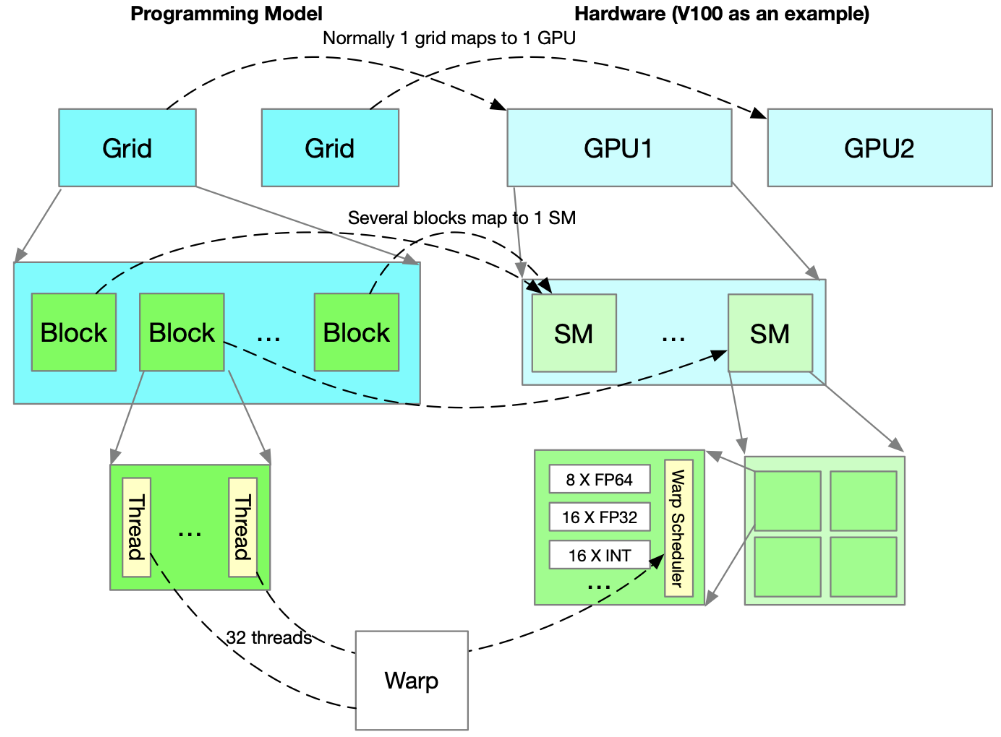
\includegraphics[width=0.8\linewidth]{img/cuda/modelandhwstruct}
\end{center}

\paragraph{Sincronizzazione a più livelli:} Le prestazioni decrescono con l'aumentare della divergenza nei warp. \textbf{Primitive di sincronizzazione} sono necessarie per evitare race conditions in cui diversi thread accedono simultaneamente alla stessa locazione di memoria. 

Si possono avere più livelli di sincronizzazione:
\begin{itemize}
	\item \textbf{System-level}: attesa che venga completato un dato task su entrambi host e device
	\begin{minted}{c}
cudaError_t cudaDeviceSynchronize(void);
	\end{minted}
	Blocca l'applicazione host finché tutte le operazioni CUDA non sono completate;
	
	\item \textbf{Block-level}: attesa che tutti i thread in un blocco raggiungano lo stesso punto di esecuzione
	\begin{minted}{c}
__device__ void __syncthreads(void);
	\end{minted}
	Sincronizza i thread all'interno di un blocco: attende fino a che tutti raggiungono il punto di sincronizzazione
	
	\item \textbf{Warp-level}: attesa che tutti i thread in un warp raggiungano lo stesso punto di esecuzione
	\begin{minted}{c}
__device__ void __syncwarp(mask);
	\end{minted}
	Sincronizza i thread all'interno di un warp: attende fino a che tutti raggiungono il punto di sincronizzazione (riconverge)
\end{itemize}

La sincronizzazione a livello di blocco va usata con attenzione, può anche portare a deadlock, un esempio semplice può essere una sincronizzazione dentro un \texttt{if-else}: potrebbero esserci thread che non entreranno mai nel ramo con la sincronizzazione, causando deadlock.

Il compilatore ha tecniche di ottimizzazione per evitare divergenza all'interno del warp (es: per un \texttt{if} calcola entrambi i branch).

\subsection{Parallel reduction}

Un'operazione comune che va sotto il nome di \textbf{reduction} è la somma di elementi di array, solitamente di grandi dimensioni. 

Per un operatore di reduction le proprietà richieste sono commutatività e associatività; con queste gli elementi possono essere riordinati e combinati in qualsiasi modo.

L'approccio sequenziale è molto semplice, in parallelo un'idea potrebbe essere:
\begin{itemize}
	\item Suddividere il vettore in parti più piccole
	
	\item Attivare i thread per la somma parziale sui pezzi 
	
	\item Sommare tra loro i risultati parziali ottenuti
\end{itemize}

Questo approccio si può implementare in due modi:
\begin{itemize}
	\item sommando le coppie di elementi contigui: al passaggio $i$ il thread \texttt{tid} somma valori a distanza $2^i$: \texttt{A[tid] + A[tid + $2^i$]}
	
	\item sommando coppie di elementi equispaziati (stride): al passaggio $i$ il thread \texttt{tid} somma elementi a distanza \texttt{len(A)/$2^{i+1}$}: \texttt{A[tid] + A[tid + len(A)/$2^{i+1}$]}
\end{itemize}

Queste presupponendo che la lunghezza del vettore sia una potenza di 2 e che $i$ parta da 0.

\paragraph{Somma strided:} La strategia parallela è simile alla somma ricorsiva con stride: 
\begin{itemize}
	\item Ad ogni passo un numero di thread pari alla metà degli elementi effettua le somme parziali (riduzione)
	
	\item Il numero di thread attivi si dimezza ad ogni passo (rinnovare la stride)
	
	\item Occorre sincronizzare il comportamento dei thread affinché al passo \texttt{t} abbiano tutti terminato il compito prima di andare al passo \texttt{t+1} (analogo alla chiamata ricorsiva) 
\end{itemize}

Un possibile codice:
\begin{minted}{c}
for (int stride = 1; stride < blockDim.x; stride *= 2) {
    if ((tid % (2 * stride)) == 0)
        idata[tid] += idata[tid + stride];
}
\end{minted}

Questa soluzione può introdurre divergenza crescente a livello di warp: i thread attivi sono "distanti" a livello di warp, nel primo passo si attivano solo i thread con indici pari, nella seconda iterazione solo la metà pari degli indici precedenti (un quarto dei thread), \dots

Vogliamo eliminare la divergenza, fondamentalmente usando thread adiacenti (quindi all'interno dello stesso warp): "convertiamo" gli indici in modo da usare sempre i \texttt{tid} più bassi possibili:
\begin{minted}{c}
for (int stride = 1; stride < blockDim.x; stride *= 2) {
    int index = 2 * stride * tid;
    if (index < blockDim.x)
        idata[index] += idata[index + stride];
    __syncthreads();
\end{minted}

Da notare come viene eliminata la clausola \texttt{if} in tutti i thread. La locazione delle somme parziali non cambia, viene modificato solo l'indice dei thread.

\subsection{Operazioni Atomiche}

Per evitare race conditions, le \textbf{operazioni atomiche} in CUDA eseguono (solo) operazioni matematiche senza interruzione da altri thread. Si tratta di funzioni che vengono tradotte in istruzioni singole.

Le operazioni basilari sono:
\begin{itemize}
	\item Matematiche: add, subtract, maximum, minimum, increment, and decrement
	
	\item Bitwise: AND, bitwise OR, bitwise XOR
	
	\item Swap: scambiano valore in memoria con uno nuovo
\end{itemize}

\subsubsection{Calcolo dell'istogramma per immagini RGB}

L'istogramma del colore è una rappresentazione della distribuzione (frequenza relativa/assoluta) tonale dei colori in un'immagine. Può essere costruito per ogni spazio colore, come RGB o HSV.

Per calcolare l'istogramma bisogna: 
\begin{itemize}
	\item Considerare separatamente i canali RGB dell'immagine
	
	\item Usare le operazioni atomiche per il calcolo delle frequenze 
	
	\item Restituire 3 istogrammi distinti (uno per canale) di 256 valori di intensità colore
\end{itemize}

L'idea è molto semplice: si alloca una struttura dati (array lungo \texttt{3 * 256}) per mantenere i valori dell'istogramma e, per ogni pixel dell'immagine si effettua una \texttt{atomicAdd()} per incrementare il valore della frequenza dei colori presenti nel pixel. 

Esempio per una immagine PPM: 
\begin{minted}{c}
__global__ void ppm_histGPU(PPM ppm, int *histogram) {
	uint x = blockIdx.x * blockDim.x + threadIdx.x;
	
	if (x >= ppm.width * ppm.height)
		return;
	
	color R = ppm.image[3 * x];
	color G = ppm.image[3 * x + 1];
	color B = ppm.image[3 * x + 2];
	
	atomicAdd(&histogram[R], 1);
	atomicAdd(&histogram[G + 256], 1);
	atomicAdd(&histogram[B + 512], 1);
}
\end{minted}

Se l'incremento non fosse atomico, un thread potrebbe venire interrotto da altri mentre tenta di incrementare una cella, possibilmente portando a race conditions e risultati inconsistenti.

\subsection{Memoria CUDA}

Per il programmatore esistono due tipi di memorie: 
\begin{itemize}
	\item \textbf{Programmabile}: controllo esplicito di lettura e scrittura per dati che transitano in memoria
	
	\item \textbf{Non programmabile}: nessun controllo sull'allocazione dei dati, gestiti con tecniche automatiche (e.g., memorie CPU e cache L1 e L2 della GPU)
\end{itemize}

Nel modello di memoria CUDA sono esposti diversi tipi di memoria programmabile: 
\begin{enumerate}
	\item registri

	\item shared memory

	\item local memory

	\item constant memory

	\item texture memory

	\item global memory
\end{enumerate}

\paragraph{Cache su GPU:} Come nel caso delle CPU, le cache su GPU \textbf{non sono programmabili}. Sono presenti 4 tipi:
\begin{itemize}
	\item \textbf{L1}, una per ogni SM
	
	\item \textbf{L2}, condivisa tra tutti gli SM
	
	\item \textbf{Read-only constant}
	
	\item \textbf{Read-only texture} (L1 da CC 5.0)
\end{itemize}

La \textbf{cache L1} è presente all'interno di ogni SM; in alcune architetture (Fermi e successive) la dimensione può essere configurata, con una porzione assegnabile a memoria condivisa. Capacità limitata ma permette di sfruttare località dei dati.

La \textbf{cache L2} ha dimensione maggiore ed è condivisa tra tutti gli SM, funziona da intermediario tra memoria globale e cache L1 dei singoli SM. Raccoglie i dati necessari a tutti gli SM e contribuisce a mantenere la coerenza dei dati tra vari SM.

L1 e L2 sono usate per memorizzare dati in memoria locale e globale, incluso lo spilling dei registri (eccessi nell'uso di local memory).

Ogni SM ha anche una \textbf{read-only constant cache} e \textbf{read-only texture cache} (non sempre fisiche) usate per migliorare le prestazioni in lettura dai rispettivi spazi di memoria sul device.

Read-only constant cache è ottimizzata per dati globali costanti condivisi tra tutti i thread, con accesso uniforme e caching efficiente. Read-only texture cache è ideale per dati in sola lettura con accesso non coalescente, sfruttando la località spaziale e offrendo funzionalità di interpolazione e filtraggio hardware.

Suddivisione fisica:
\begin{center}
	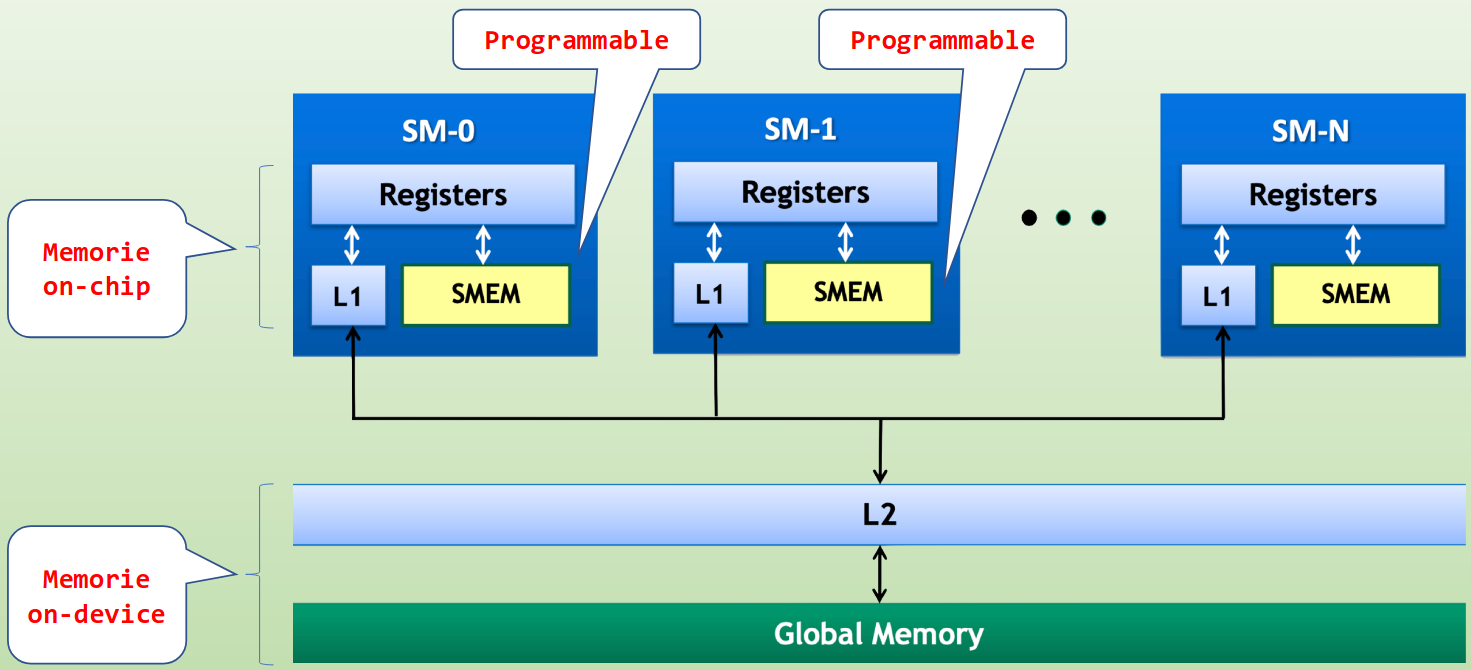
\includegraphics[width=0.85\linewidth]{img/cuda/mem1}
\end{center}

Nel tempo, è stata gradualmente aumentata la dimensione delle cache L1 e L2, allo stesso tempo incrementando la memoria condivisa tra gli SM, fino all'introduzione di una L0 instruction cache in Volta, oltre a 128kB di cache L1 unita alla shared memory (smem).

\subsubsection{Cooperating Threads/Shared Memory}

Un blocco può avere della \textbf{memoria condivisa} e tutti thread all'interno del blocco hanno la stessa visuale su questa memoria; la memoria è unica per blocco e inaccessibile ad altri blocchi. Viene dichiarata tramite \texttt{\_\_shared\_\_}.

La SMEM è suddivisa in moduli della stessa ampiezza, chiamati \textbf{bank}. Ogni richiesta di accesso fatta di $n$ indirizzi che riguardano $n$ distinti bank sono serviti simultaneamente.

Ogni SM ha una quantità limitata di shared memory che viene ripartita tra i blocchi di thread. La smem serve come base per la comunicazione inter-thread: i thread all'interno di un blocco possono cooperare scambiandosi dati memorizzati in shared memory. L'accesso deve essere sincronizzato per mezzo di \texttt{syncthreads()}.

\paragraph{Organizzazione fisica:} La smem è suddivisa in blocchi da 4 byte (word), ogni accesso legge almeno la word di appartenenza (anche se viene richiesto un solo byte).

Dati 32 bank, ogni word è memorizzata in bank distinti, a gruppi di 32. Dato l'indirizzo del byte: 
\begin{itemize}
	\item diviso 4 si ottiene l'indice della word

	\item l'indice della word modulo $32$ è l'indice della bank
\end{itemize}

\paragraph{Smem a runtime:} La memoria viene ripartita tra tutti i blocchi residenti in un SM. Maggiore è la shared memory richiesta da un kernel, minore è il numero di blocchi attivi concorrenti. 

Il contenuto della shared memory ha lo stesso lifetime del blocco a cui è stata assegnata.

\paragraph{Pattern di accesso:} Se un'operazione di \texttt{load} o \texttt{store} eseguita da un warp richiede al più un accesso per bank, si può effettuare in una sola transizione il trasferimento dei dati dalla shared memory al warp. In alternativa sono richieste diverse ($\leq 32$) transazioni, con effetti negativi sulla bandwidth globale.

L'accesso ideale è una singola transazione per warp.

Ci possono essere dei \textbf{conflitti}: un \textbf{bank conflict} accade quando si hanno diversi indirizzi di shared memory che insistono sullo stesso bank.

L'hardware effettua tante transazioni quante ne sono necessarie per eliminare i conflitti, diminuendo la bandwidth effettiva di un fattore pari al numero di transazioni separate necessarie (vengono serializzati gli accessi).

\paragraph{Osservazioni:}
\begin{itemize}
	\item \textbf{Latency hiding}: il ritardo tra richiesta dei thread alla smem e l'ottenimento dei dati, in generale, non è un problema, anche in caso di bank conflict; lo scheduler passa a un altro warp in attesa che quelli sospesi completino il trasferimento dei dati dalla smem
	
	\item \textbf{Inter-block}: non esiste conflitto tra thread appartenenti a blocchi differenti, il problema sussiste solo a livello di warp dello stesso blocco 
	
	\item \textbf{Efficienza massima}: il modo più semplice per avere prestazioni elevate è quello di fare in modo che un warp acceda a word consecutive in memoria shared
	
	\item \textbf{Caching}: con scheduling efficace, le prestazioni (anche in presenza di conflitti a livello smem) sono molto migliori rispetto alla cache L2 o global memory
\end{itemize}

\subsubsection{Allocazione della SMEM}

\paragraph{Allocazione statica:} Una variabile in shared memory può anche essere dichiarata locale a un kernel o globale in un file sorgente. Viene dichiarata con il qualificatore \texttt{\_\_shared\_\_}. Può essere dichiarata sia staticamente sia dinamicamente. 

Se statica, può essere 1D, 2D o 3D, con dimensione nota compile time.

\paragraph{Allocazione dinamica:} Per allocare la shared memory dinamicamente (in bytes), occorre indicare un terzo argomento all'interno della chiamata del kernel:
\begin{minted}{c}
kernel <<<grid, block, N*sizeof(int)>>>(...)
\end{minted}

Se la dimensione non è nota compile time, è possibile dichiarare una variabile adimensionale con la keyword \texttt{extern}. Dinamicamente si possono allocare solo array 1D.

\paragraph{Allocazione dinamica multipla:} Non si possono allocare multiple allocazioni di shared memory, quindi bisogna fare un'allocazione unica e utilizzare puntatori con offset all'interno dell'area allocata.

Uso tipico della shared memory:
\begin{enumerate}
	\item Carica i dati dalla device memory alla shared memory
	
	\item Sincronizza i thread del blocco al termine della copia che ognuno effettua sulla shared memory (così che ogni thread possa elaborare dati certi andando avanti)
	
	\item Elabora i dati in shared memory

	\item Sincronizza (se necessario) per essere certi che la shared memory contenga i risultati aggiornati
	
	\item Scrivi i risultati dalla device memory alla host memory
\end{enumerate}

\subsubsection{Prodotto Convolutivo con SMEM}
La \href{https://it.wikipedia.org/wiki/Convoluzione}{\texttt{convoluzione}} sono una serie di somme e prodotti
$$ y(n) = h(n) \cdot x(n) = \sum_{k=0}^{N-1} h(k) x(n-k) $$

Si prende un segnale, si considera un kernel/finestra su tale segnale, si fanno i prodotti. Il tutto viene fatto un numero \textit{molto elevato} di volte. Si può scalare il processo a più dimensioni.

Ci sono sempre problemi di bordo: cosa faccio quando la maschera considerata arriva al bordo dei dati? Andrebbe fuori, quindi devo popolare nel modo corretto i dati mancanti (\texttt{0}? Li invento?).

\paragraph{Tiling:} Divido i dati in blocchi (ad esempio, 16 elementi in 4 blocchi da 4 thread), ogni thread nel blocco fa un prodotto della convoluzione. Per ridurre l'accesso alla global memory, in cache/memoria condivisa si tengono i dati a cui l'accesso è fatto più frequentemente, ovvero i valori del "blocco di dati" assegnato al block (tutti i thread devono calcolare sullo stesso insieme di dati, o quasi), tenendo conto della dimensione della maschera (serve avere i dati "adiacenti" al blocco (sarebbe molto utile un'immagine, si capirebbe subito)).

I dati da caricare in smem sono più dei thread nel blocco ("alone" che va al di fuori del blocco di dati stesso); in smem carico tutti i possibili dati a cui il blocco deve fare l'accesso. Chi carica che dati in memoria? I dati esterni al blocco potrebbero essere anche più del blocco stesso (maschera "grossa"). La soluzione è dare un ordine ai thread e dividere il più equamente possibile i caricamenti in memoria tra i thread del blocco.

\subsubsection{Prodotto matriciale con SMEM}

L'approccio più ovvio è quello di lasciare a ogni thread il calcolo di una cella della matrice prodotto. Ogni blocco si occuperebbe di una sezione della matrice prodotto risultante. 

In memoria condivisa andrebbero caricate tutte le righe e colonne delle matrici da cui fare il prodotto. Per distribuire equamente il lavoro tra i thread, si può fare tiling anche delle aree da caricare (multiple della dimensione del blocco, se definite correttamente/le dimensioni in ingresso lo permettono). Una volta finito il caricamento e la sincronizzazione a livello di blocco, ogni thread può calcolare la sua entry della matrice.

Pseudocodice del kernel:
\begin{center}
	\begin{minipage}{.9\textwidth}
		\begin{tcolorbox}[
			colback=white,
			sharp corners,
			boxrule=.3mm,
			left=20pt,
			top=0pt,
			bottom=0pt,
			colbacktitle=white,
			coltitle=black
			]
			\LinesNumbered
			\begin{algorithm}[H]
				\SetAlgoNoEnd
				\SetKwSty{texttt}
				\SetArgSty{relax}
				\texttt{\_\_shared\_\_ As[WIDTH][WIDTH]}; \\
				\texttt{\_\_shared\_\_ Bs[WIDTH][WIDTH]}; \\
				\texttt{nblocks =} numero di block nelle sotto-matrici da caricare; \\
				\For{$i \in$ \texttt{nblocks}}{
					\texttt{As[tidy][tidx] = A[tidx\_abs + $i$ * WIDTH][tidy\_abs]}; \\
					\texttt{Bs[tidy][tidx] = B[tidx\_abs][tidy\_abs + $i$ * WIDTH]}; \\
					\texttt{\_\_syncthreads()}; \\
					
					\For{$j \in$ \texttt{WIDTH}}{
						\texttt{partial\_sum += As[tidy][j] * Bs[j][tidx]}; \\
					}
					\texttt{\_\_syncthreads()};\\
				}
				\tcp*{Srivere il risultato in memoria globale}
			\end{algorithm}
		\end{tcolorbox}
	\end{minipage}
\end{center}

L'idea è: 
\begin{itemize}
	\item Caricare il primo tile
	
	\item Effettuare la somma parziale per ogni cella
	
	 \item Ripetere per il numero di tile contenuti nelle zone delle matrici da caricare
	 
	 \item Scrivere i risultati finali in memoria globale
\end{itemize}

\subsection{Global Memory}

Nei computer moderni esiste una gerarchia di memorie per minimizzare latenze e massimizzare throughput. In genere, si ha l'illusione virtuale di una grande memoria, tutta a bassa latenza, anche se la memoria con effettivamente bassa latenza è poca e si ha una memoria ad alta capacità e alta latenza.

All'interno delle GPU abbiamo, dalla latenza più alta alla più bassa: 
\begin{itemize}
	\item Device Memory
	
	\item L2 Cache
	
	\item L1/shared
	
	\item Registers
\end{itemize}

Le gerarchie di memorie, comprese quelle CUDA, fanno fede ai principi di: 
\begin{itemize}
	\item \textbf{Località spaziale}: se l'istruzione all'indirizzo $i$ viene eseguita, probabilmente dopo verrà eseguita quella all'indirizzo $i + \Delta i$
	
	\item \textbf{Località temporale}: se un'istruzione viene eseguita al tempo $t$, probabilmente verrà eseguita anche al tempo $t + \Delta t$ (dove $\Delta t$ è piccolo)
\end{itemize}

\paragraph{Registers:} Le memorie più veloci in assoluto, con lifetime del kernel. Vengono ripartiti tra i warp attivi, le variabili dichiarate nel codice device senza qualificatori generalmente risiedono in un registro. 

Meno registri usa il kernel, più blocchi di thread è probabile che risiedano sull'SM (il compilatore usa un'euristica per ottimizzare questo parametro). \textbf{Register spilling}: se si usano più registri di quelli consentiti le variabili si riversano nella local memory.

\paragraph{Local Memory:} Si tratta di una memoria \textit{lenta} (collocata off-chip, alta latenza, bassa bandwidth). Si tratta di una memoria locale ai thread.

Usata per contenere le variabili automatiche (grandi) non contenute nei registri, o per le variabili al di fuori causa spilling. La local memory risiede nella device memory, pertanto gli accessi hanno stessa latenza e ampiezza di banda della global memory e sono soggetti anche agli stessi vincoli di coalescenza-

Da CC 2.0 ci sono parti poste in cache L1 a livello di SM e in cache L2 a livello di device. Il compilatore \texttt{nvcc} si preoccupa della sua allocazione e non è controllata dal programmatore.

\paragraph{Constant Memory:} Risiede nella device memory (64K per tutte le CC) ed ha una cache dedicata in ogni SM (8K). Definibile tramite l'attributo \texttt{\_\_constant\_\_}. 

Ospita dati in sola lettura, ideale per accessi uniformi. Ha scope globale, va dichiarata al di fuori di qualsiasi kernel e viene dichiarata staticamente, quindi è visibile a tutti i kernel nella stessa unità di compilazione.

La constant memory può essere inizializzata dall'host usando:
\begin{minted}{c}
cudaError_t cudaMemcpyToSymbol(const void* symbol,
    const void* src, size_t count)
\end{minted}

Lavora bene quando tutti i thread di un warp leggono dallo stesso indirizzo di memoria (raggiunge l'efficienza dei registri); se i thread di un warp leggono da indirizzi diversi allora le letture vengono serializzate, riducendo l'efficienza.

\paragraph{Texture Memory:} Risiede nella device memory e (può avere) una read-only cache per-SM ed è acceduta solo attraverso di essa. La cache include un supporto hardware efficiente per filtraggio o interpolazione floating-point nel processo di lettura dei dati. 

Ottimizzata per la località spaziale 2D, quindi dati espressi sotto forma di matrici. I thread in un warp che usano la texture memory per accedere a dati 2D hanno migliori prestazioni rispetto a quelle standard, quindi è adatta per applicazioni in cui servono classiche elaborazioni di immagini/video. Per altre applicazioni l’uso della texture memory potrebbe essere più lento della global memory.

\paragraph{Global Memory:} La più grande, con più alta latenza e più comunemente usata memoria su GPU. Ha scope e lifetime globale (da qui il nome). Dichiarazione (codice host):
\begin{center}
	\begin{tabular}{r | l r | }
		\cline{2-3}
		\textbf{Statica} & \texttt{\_\_device\_\_ int a[N];} & \\
		\textbf{Dinamica} & \texttt{cudaMalloc((void **)\&d\_a, N);} & \texttt{cudaFree(d\_a);} \\
		\cline{2-3}
	\end{tabular}
\end{center}

Corrisponde alla memoria fisica, con "global" si intende una divisione logica. L'accesso da parte di thread appartenenti a blocchi distinti può potenzialmente portare a modifiche incoerenti. La global memory è accessibile attraverso transazioni da 32, 64, o 128 byte; le transazioni avvengono solo per gruppi di valori, non si può accedere a un valore singolo.

I valori contenuti nella memoria allocata non sono inizializzati, ma si possono inizializzare con dati provenienti dall'host (\texttt{cudaMemcpy}) oppure con un valore specifico
\begin{minted}{c}
cudaError_t cudaMemset(void* devPtr, int value, size_t count)
\end{minted}

Assegna il valore \texttt{value} a tutti gli indirizzi contenuti nel blocco di memoria.

La memoria allocata è opportunamente allineata per ogni tipo di variabile. La \texttt{cudaMalloc} restituisce \texttt{cudaErrorMemoryAllocation} in caso di fallimento.

Lo \textbf{specificatore \texttt{\_\_device\_\_}} indica una variabile che risiede unicamente sul device. Risiede nella memoria globale (e quindi oggetti distinti per device diversi), ha il lifetime del contesto CUDA in cui è stata creata. Può essere acceduta da tutti i thread e dall'host tramite la libreria runtime:
\begin{itemize}
	\item \texttt{cudaGetSymbolAddress()}, \texttt{cudaGetSymbolSize()}: per ottenere indirizzo e dimensione di una variabile, rispettivamente
	
    \item \texttt{cudaMemcpyToSymbol()}, \texttt{cudaMemcpyFromSymbol()}: per copiare verso e da una variabile, rispettivamente
\end{itemize}

Riassunto dichiarazione di variabili: 
\begin{center}
	\begin{tabular}{|l|l|l|l|l|}
		\hline
		\textbf{QUALIFIER} & \textbf{VARIABLE} & \textbf{MEMORY} & \textbf{SCOPE} & \textbf{LIFESPAN} \\
		\hline
		& \texttt{float var} & Register & Local & Thread \\
		\hline
		& \texttt{float var[100]} & Local & Local & Thread \\
		\hline
		\texttt{\_\_shared\_\_} & \texttt{float var} & Shared & Block & Block \\
		\hline
		\texttt{\_\_device\_\_} & \texttt{float var} & Global & Global & Application \\
		\hline
		\texttt{\_\_constant\_\_} & \texttt{float var} & Constant & Global & Application \\
		\hline
	\end{tabular}
\end{center}

\subsection{Pinned memory}
La pinned memory (o page-locked memory) in CUDA è una tecnica che serve per ottimizzare il trasferimento dei dati tra la memoria del sistema (RAM) e la memoria della GPU (VRAM). 

Si vuole evitare il page fault della virtual memory (CPU, di default la memoria host allocata è paginabile). Esistono delle primitive per definire una memoria pinned, ovvero viene tolta la pagina dal meccanismo di virtualizzazione in modo che l'host non possa "toglierla" mentre il device la deve usare. Blocca la memoria in modo da poter fare trasferimenti asincroni al device.

Una volta "pinnata", la memoria non sparirà dal sistema di virtualizzazione automatico della memoria host, quindi si può lavorare su quella memoria in maniera asincrona. La pinned memory può essere acceduta direttamente dal device, in modalità asincrona. Può essere letta e scritta con una bandwidth più alta rispetto alla memoria paginabile.

Da notare che eccessi di allocazione di pinned memory potrebbero far degradare le prestazioni dell'host (ridurre la memoria paginabile inficia l'uso della virtual memory), Per allocare esplicitamente memoria pinned:
\begin{minted}{c}
cudaError_t cudaMallocHost(void **devPtr, size_t count);
\end{minted}

E per deallocarla:
\begin{minted}{c}
cudaError_t cudaFreeHost(void *devPtr);
\end{minted}

Questa allocazione sostituisce la malloc "normale", su host. Rende i trasferimenti host-device significativamente più veloci, al costo di un tempo più alto di allocazione.

\subsection{Unified Virtual Addressing UVA}

Si vuole avere un unico spazio di indirizzamento tra CPU e tutte le GPU. Tutti i puntatori (CPU e GPU) appartengono allo stesso spazio di indirizzi virtuali, di conseguenza è possibile passare un puntatore da host a device e viceversa senza ambiguità, entrambi possono "capire" a cosa punta quell'indirizzo.

% End L5

La unified memory è una memoria "\textit{comoda}", fornisce un puntatore unico per tutte le CPU e GPU presenti nel sistema. Spazio di indirizzamento unico per CPU e GPU.

Con "\textbf{Managed Memory}" si fa riferimento ad allocazioni della unified memory. All'interno di un kernel si possono usare entrambi i tipi di memoria: 
\begin{itemize}
	\item managed memory, controllata dal sistema
    
	\item un-managed memory, controllata esplicitamente dall'applicazione
\end{itemize}

Tutte le operazioni CUDA valide sulla memoria del dispositivo sono valide anche sulla memoria managed.

Per fare allocazione dinamica:
\begin{minted}{c}
cudaError_t cudaMallocManaged(void **devPtr, size_t size, 
    unsigned int flags=0)
\end{minted}

"rimpiazza" \texttt{cudaMalloc}, la \texttt{flag} indica chi condivide il puntatore con il device:
\begin{itemize}
	\item \texttt{cudaMemAttachHost}: solo la CPU
    
	\item \texttt{cudaMemAttachGlobal}: anche tutte le altre GPU
\end{itemize}

Nuova \textbf{keyword}: \textbf{\texttt{\_\_managed\_\_}}, si tratta di un qualifier che denota scope globale, accessibile da CPU e GPU.

Con l'uso "misto" di memoria bisogna porre attenzione alla sincronizzazione tra CPU e GPU, onde evitare problemi.

\subsection{Pattern di Accesso alla Global Memory}

Gli accessi alla memoria del dispositivo possono avvenire in transazioni da 32, 64 o 128 byte. Le applicazioni GPU tendono (a volte) ad essere limitate dalla memory bandwidth, quindi massimizzare il throughput effettivo è importante. 

In generale, per rendere efficienti le transazioni in memoria:
\begin{itemize}
	\item minimizzare il numero di transazioni per servire il massimo numero di accessi
    
	\item considerare che il numero di transazioni e throughput ottenuto variano con la CC
\end{itemize}

Per migliorare le prestazioni in lettura e scrittura occorre ricordare che: 
\begin{itemize}
	\item le istruzioni vengono eseguite a livello di warp e gli accessi in memoria dipendono dalle operazioni svolte nel warp
    
	\item per un dato indirizzo si esegue un'operazione di loading o storing (gestione diversa)
	
    \item i 32 thread presentano una singola richiesta di accesso, che viene servita da una o più transazioni in memoria
\end{itemize}

In base a come sono distribuiti gli indirizzi di memoria, gli accessi alla stessa possono essere classificati in pattern distinti. Tutti gli accessi a memoria globale passano dalla cache L2, molti passano anche dalla L1. Se entrambe le memorie vengono usate gli accessi sono da 128 byte, altrimenti, se viene usata solo la L2, gli accessi sono a 32 byte.

Per le architetture che usano cache L1, queste possono essere esplicitamente abilitate o disabilitate a compile time.

Bisogna rispettare allineamento e coalescenza per sfruttare al meglio le transazioni di memoria; per avere accessi in memoria efficienti è necessario combinare in un unica transazione accessi multipli a memoria allineati e coalescenti.

Accesso \textbf{allineato}: quando il primo indirizzo della transazione è un multiplo pari della granularità della cache che viene usata per servire la transazione (32 byte per la cache L2 o 128 byte per la cache L1).

Accesso \textbf{coalescente:} quando tutti i 32 thread in un warp accedono a un blocco contiguo di memoria.

In un SM i dati seguono pipeline attraverso i seguenti tre cache/buffer paths dipendentemente da quale tipo di device memory si accede:
\begin{itemize}
	\item L1/L2 cache
    
	\item Constant cache
	
    \item Read-only cache
\end{itemize}

L1/L2 cache rappresenta il default path. Il fatto che un'operazione di \texttt{load} in global memory passi attraverso la cache L1 dipende da CC e compiler options.

\paragraph{Scritture:} Le write vengono servite in modo diverso, non viene usata la cache L1, ma le \texttt{store} sono cachate solo in L2, prima di essere inviate alla device memory in segmenti da 32 byte; vengono trasferiti 1,2 o 4 segmenti alla volta.

Quando forzati a fare accessi (letture/scritture) non coalescenti si può usare la shared memory come "passaggio" per rendere le operazioni effettive in memoria coalescenti.

\paragraph{AoS vs SoA:} I dati possono essere divisi in: 
\begin{itemize}
	\item \textbf{Array of Structures AoS}:
	\begin{minted}{c}
struct Particle { float x, y, z; };
Particle* P;
float x = P[idx].x;  // stride = sizeof(Particle)
	\end{minted}
	Questo porta a distanza tra accessi (stride) alta, rompendo la coalescenza
	
	\item \textbf{Structure of Arrays SoA}:
	\begin{minted}{c}
float *Px, *Py, *Pz;
float x = Px[idx];   // stride = 1
	\end{minted}
	In questo modo lo stride è ridotto, riducendo così il numero di transazioni necessarie
\end{itemize}

\paragraph{TL;DR:} Un warp può effettuare accessi
\begin{itemize}
	\item coalescenti: i 32 thread leggono dati contigui, massima efficienza
	\item non coalescenti/strided: dati a distanza $>1$, possono servire più transazioni per la stessa quantità di dati, fino a 32 diverse
\end{itemize}

In generale (per CC superiori a 2) le transazioni coprono 128 byte. All'interno di un singolo segmento da 128 byte, la memoria è organizzata in "banks" (4 da 32 byte solitamente), anche se un thread legge solo 4 byte, dovrà trasferire l'intero bank.

La cache L1 serve load/store anche con granularità a 32 byte.

\subsubsection{Matrice trasposta con SMEM}

Il problema del parallelizzare l'operazione di trasposizione di una matrice  è che in lettura gli accessi sono per riga, quindi coalescenti, mentre le scritture sulla matrice trasposta sono per colonna, quindi non coalescenti.

Un'idea per risolvere il problema può essere: 
\begin{itemize}
	\item Caricare dalla global memory alla smem le celle che il blocco corrente deve trasporre, riga per riga
	
	\item Leggere una colonna in smem e scrivere una riga in global memory
\end{itemize}

Esempio:
\begin{minted}{c}
__shared__ float tile[BDIMY][BDIMX];
// Coordinate originali
unsigned int row = blockDim.y * blockIdx.y + threadIdx.y;
unsigned int col = blockDim.x * blockIdx.x + threadIdx.x;

// ...
// Trasferimento in smem e sincronizzazione

// Nuovi indici
int y = blockIdx.x * blockDim.x + threadIdx.y;
int x = blockIdx.y * blockDim.y + threadIdx.x;

// ...
// Scrivere sulla matrice output, 
//		controlli invertiti tra riga e colonna
\end{minted}

	% !TeX spellcheck = it_IT
\section{Ottimizzazione delle Prestazioni}

\subsection{Risorse Hardware}

\paragraph{Device Query:} Per indagare le feature disponibili sul device, scoprire le proprietà. Ad esempio: quanti SM sono disponibili, quanta memoria, \dots\\

Per farlo ci sono \href{http://docs.nvidia.com/cuda/cuda-runtime-api}{\texttt{Funzioni delle API runtime di CUDA}} e la CLI utility \href{https://developer.nvidia.com/nvidia-system-management-interface}{\texttt{nvidia-smi}}. Quest'ultimo permette di gestire e monitorare le GPU presenti.\\

Le funzioni: 
\begin{center}
	\texttt{cudaError\_t cudaGetDeviceCount(\&dev\_count)} \\
	\texttt{cudaError\_t cudaGetDeviceProperties(cudaDeviceProp* prop, int device);}
\end{center}
Indaga il numero di device disponibili sul sistema e restituisce le proprietà del device nella struttura \texttt{cudaDeviceProp} (rispettivamente).\\

%TODO
\subsection{Gestione ottimizzata delle risorse}

L'ottimizzazione delle performance si basa su 4 strategie principali:
\begin{itemize}
	\item massimizzare l'utilizzazione tramite massimo parallelismo
	\item ottimizzare l'utilizzo di memoria per avere il throughput di memoria massimo
	\item ottimizzare l'uso di istruzioni per avere il massimo throughput
	\item minimizzare il memory thrashing
\end{itemize}

Che strategie permettono di ottenere le migliori performance per una determinata applicazione dipende da qual'è il fattore limitante all'interno dell'applicazione stessa. Gli sforzi per l'ottimizzazione vanno quindi costantemente direzionati monitorando i fattori che limitano le performance, tramite strumenti come il CUDA profiler. \\

\newpage

\paragraph{Register spilling:} Il massimo numero di registri per thread può essere definito manualmente compile time con l'opzione \texttt{-maxrregcount} e si può indagare (sempre compile time) con \texttt{--ptxas-options=-v}. \\
Limitare il numero porta a fare spilling (quindi usare la memoria locale), ma aumentando il numero di blocchi concorrenti. \\ %(maybe)

\subsection{Profiling}

Nvidia mette a disposizione dei \textbf{developer tools} per effettuare profiling e monitorare le applicazioni. \\

\paragraph{Nsight Compute:} Profiler di livello kernel che fornisce informazioni dettagliate sulle metriche di esecuzione dei kernel CUDA. Permette una misurazione dettagliata delle prestazioni dei kernel (latency, throughput, utilizzo delle risorse, ecc.), analisi delle performance a livello di istruzione e accesso alla memoria, supporto per personalizzare la raccolta di metriche e approfondire l’ottimizzazione delle singole funzioni CUDA. \texttt{ncu, ncu-ui}, CLI e GUI.\\

\paragraph{Nsight Systems:} Offre un'analisi a livello di sistema, ideale per identificare bottleneck nell'interazione tra CPU e GPU. Fornisce una visione d’insieme dell'intero flusso applicativo, monitorando la sincronizzazione tra processi e thread, il trasferimento dei dati e l'esecuzione complessiva. Permette di analizzare come le attività CUDA si integrino con il resto dell'applicazione, evidenziando le possibili ottimizzazioni per bilanciare meglio l’utilizzo di tutte le risorse hardware. \texttt{nsys, nsys-ui}, CLI e GUI.\\

\newpage

%back to main slides
\subsection{Loop Unrolling}
Il loop unrolling può essere utile per ottimizzare i cicli: questi vengono espansi ("srotolati") in modo da ridurre l'effettivo numero di iterazioni necessarie durante l'esecuzione del kernel. Il corpo del ciclo viene riscritto più volte. \\

Questo ha diversi vantaggi, tra cui: 
\begin{itemize}
	\item riduzione dell'overhead dovuto ai controlli del ciclo
	\item eliminazione di salti e riduzione della logica di controllo 
	\item aumento del livello di parallelismo
\end{itemize}

Il numero di copie del corpo del loop create si chiama \textbf{unrolling factor} (quanto è stato "srotolato" il ciclo). Questa tecnica è efficace quando il numero di iterazioni è noto a priori.\\

\paragraph{Warp unrolling:} L'ottimizzazione si può anche migliorare sfruttando il concetto di warp. Tutti i 32 thread all'interno di un solo warp eseguono lo stesso codice in maniera sincrona, si usa questa caratteristica per unrollare il codice di un ciclo in maniera esplicita, eliminando controlli ed eventuali divergenze tra thread. Dato che tutti gli warp eseguono lo stesso codice, l'unrolling garantisce che il flusso di esecuzione rimanga uniforme, riducendo la divergenza (percorsi di codice differenti all'interno del medesimo warp). \\

% End L6

\subsection{Parallelismo dinamico}

Ci siamo mai chiesti se si può lanciare un kernel all'interno di un kernel? Not really, ma potrebbe essere utile (come ad esempio per la ricorsione). Nuova feature introdotta dalle CC 3.5: ogni kernel può lanciare un altro kernel e gestire dipendenze inter-kernel. Elimina la necessità di comunicare con la CPU, rende più semplice creare e ottimizzare pattern di esecuzione ricorsivi e data-dependent. Senza parallelismo dinamico la CPU deve lanciare ogni kernel.\\

L'idea dietro il parallelismo dinamico è generare dinamicamente kernel in base ai dati: se ci sono elementi diversi/zone della matrice di lavoro che richiedono sforzi diversi possiamo fare in modo che i kernel sian \textit{ad hoc} per migliorare l'efficienza.\\

%Esempio: Mandelbrot %Ci saranno le slide, forse, da qualche parte

Senza permettere al kernel di lanciare altri kernel il modello di esecuzione è inefficiente: la CPU non può essere conscia dei dati, ma è lei che deve lanciare \textit{tutti} i kernel, la GPU valuta se è necessario lanciare nuovi kernel (in base ai dati) e tali informazioni vanno passate nuovamente alla CPU per lanciare nuovi kernel.\\

La soluzione è il \textbf{parallelismo dinamico}: la GPU può lanciare nuovi kernel, permette di ridurre la dipendenza dalla CPU e migliorare il throughput del kernel (se fatto bene). Consente carichi di lavoro dinamici senza penalizzare le prestazioni.\\

Vogliamo mettere carico di lavoro dove serve, scegliere la granularità del lavoro in base ai dati. Possiamo posporre la decisione delle dimensioni di blocchi e griglia fino a runtime. Possiamo adattare il lavoro in base a \textbf{decisioni data-driven}, non da schemi fissi come visto fino ad ora.\\

Esempio: un kernel figlio viene chiamato all'interno di un kernel padre e quest'ultimo può utilizzare i risultati prodotti dal figli senza nessuna interazione da parte della CPU
\begin{minted}{c}
__global__ ChildKernel(void* data) {
	//Operate on data
}
__global__ ParentKernel(void* data) {
	ChildKernel<<<16, 1>>>(data);
}
// In Host Code
ParentKernel<<<256, 64>>(data);
\end{minted}

Sarebbe da limitare un attimo l'annidamento: se ogni thread facesse una chiamata a kernel figlio \textit{potrebbero} diventare tanti kernel lanciati; sarebbe carino inserire \textbf{control flow attorno ai lanci}, per esempio limitando il lancio ad 1 per blocco del padre (\texttt{threadIdx.x == 0}).\\

\paragraph{Sincronizzazione:} Si ha una sincronizzazione implicita, il padre non può terminare prima dei figlio, un kernel non è considerato completato finché ha figli attivi. Rimane la possibilità di avere sincronizzazione esplicita, altrimenti il kernel padre non ha garanzie di poter vedere i dati elaborati dal figlio. \\

%Slide 7

\subsection{Librerie CUDA}
Le librerie sono comode e quelle CUDA sono accelerate dalla GPU. Le API di molte di queste sono volutamente simili a quelle della libreria standard. Permettono porting di codice da sequenziale a parallelo con \textit{minimo sforzo}, nessun tempo di mantenimento della libreria.\\

Esempi di librerie CUDA:
\begin{center}
	\begin{tabular}{@{} ll @{}}
		\hline
		\textbf{Libreria}                     & \textbf{Dominio}                                    \\ \hline
		cuFFT (NVIDIA)                        & Fast Fourier Transforms Linear                      \\
		cuBLAS (NVIDIA)                       & Linear Algebra (BLAS Library)                       \\
		cuSPARSE (NVIDIA)                     & Sparse Linear Algebra                               \\
		cuRAND (NVIDIA)                       & Random Number Generation                            \\
		NPP (NVIDIA)                          & Image and Signal Processing                         \\
		CUSP (NVIDIA)                         & Sparse Linear Algebra and Graph Computations        \\
		CUDA Math Library (NVIDIA)            & Mathematics                                         \\
		Trust (terze parti)                   & Parallel Algorithms and Data Structures             \\
		MAGMA (terze parti)                   & Next generation Linear Algebra                      \\ \hline
	\end{tabular}
\end{center}

\paragraph{Workflow tipico:} Per l'utilizzo di una libreria CUDA, il workflow generico è:
\begin{enumerate}
	\item Creare un \textbf{handle} specifico della libreria (per la gestione delle informazioni e relativo contesto in cui essa opera, es. uso degli stream)
	\item \textbf{Allocare la device memory} per gli input e output alle funzioni della libreria (convertirli al formato specifico di uso della liberia, es. converti array 2D in column-major order)
	\item \textbf{Popolare con i dati} nel formato specifico
	\item \textbf{Configurare} le computazioni per l'esecuzione (es. dimensione dei dati)
	\item Eseguire la \textbf{chiamata della funzione} di libreria che avvia la computazione sulla GPU
	\item \textbf{Recuperare i risultati} dalla device memory
	\item Se necessario, \textbf{(ri)convertire i dati} nel formato specifico o nativo dell'applicazione
	\item \textbf{Rilasciare le risorse} CUDA allocate per la data libreria
\end{enumerate}

\subsubsection{cuBLAS - Basic Linear Algebra Subproblems}

Usata per calcolo scientifico ed ingegneristico per problemi di algebra lineare numerica
\begin{itemize}
	\item risoluzione di sistemi lineari
	\item ricerca di autovalori e/o autovettori
	\item calcolo della SVD (valori e vettori singolari)
	\item fattorizzazione di matrici
\end{itemize}

Come BLAS, le funzioni di cuBLAS sono divisi in livelli: 
\begin{itemize}
	\item Livello 1: per operazioni vettore-vettore
	\item Livello 2: per operazioni vettore-matrice
	\item Livello 3: per operazioni matrice-vettore
\end{itemize}

Usa \textbf{column-major order} (leggo le colonne dall'alto verso il basso) perché chiunque ha scritto la libreria è stronzo (colpa di Fortran). Esempio: 
$$
\left[
\begin{array}{c c c}
	1 & 2 & 3 \\
	4 & 5 & 6 \\
	7 & 8 & 9
\end{array}
\right]
\rightarrow \left[\begin{array}{c c c c c c c c c}
	1 & 4 & 7 & 2 & 5 & 8 & 3 & 6  & 9
\end{array}\right]
\quad I(r,c) = c \cdot M  + r 
$$
Dove $(r,c)$ sono le coordinate del valore cercato e $M$ è l'altezza della matrice (dimensioni $M \times N$).\\

\paragraph{Operare con cuBLAS:} L'iter tipico per usare cuBLAS è 
\begin{enumerate}
	\item creare un handle con \texttt{cublasCreateHandle}
	\item allocare la memoria sul device con \texttt{cudaMalloc}
	\item poplare la device memory con gli input necessari usando \texttt{cublasSetVector} e \texttt{cublasSetMatrix}
	\item effettuare le chiamate di libreria necessarie
	\item recuperare i risultati dalla device memory usando \texttt{cublasGetVector} e \texttt{cublasGetMatrix}
	\item rilasciare le risorse CUDA e cuBLAS con \texttt{cudaFree} e \texttt{cublasDestroy}, rispettivamente
\end{enumerate}

\paragraph{Funzioni all'interno di cuBLAS:} Per trasferire vettori da CPU a GPU:
\begin{itemize}
	\item Copia \texttt{n} elementi di dimensione \texttt{elemSize} da \texttt{cpumem} sulla CPU ad un vettore \texttt{gpumem} sulla GPU
	\begin{minted}{c}
cublasSetVector(int n, int elemSize, const void *cpumem, 
	int incx, void *gpumem, int incy)
	\end{minted}
	\item L'inverso di prima (da GPU a CPU)
	\begin{minted}{c}
cublasGetVector(int n, int elemSize, const void *gpumem, 
	int incx, void *cpumem, int incy)
	\end{minted}
\end{itemize}

Per trasferire matrici (sempre column-major order): 
\begin{itemize}
	\item copia una matrice \texttt{rows} $\times$ \texttt{cols}, di elementi grossi \texttt{elemSize}, da \texttt{A} nella memoria CPU a \texttt{B} nella memoria GPU
	\begin{minted}{c}
cublasSetMatrix(int rows, int cols, int elemSize, 
	const void *A, int lda, void *B, int ldb)
	\end{minted}
	esiste anche il corrispettivo \texttt{cublasGetMatrix()} che fa l'inverso
	\item come \texttt{cublasGetMatrix()}, ma asincrono (rispetto all'host), usando il parametro \texttt{stream} fornito
	\begin{minted}{c}
cublasGetMatrixAsync(int rows, int cols, int elemSize, 
	const void *A, int lda, void *B, 
	int ldb, cudaStream_t stream)
	\end{minted}
\end{itemize}

Per gestire la libreria serve un \textbf{handle}, il quale si può generare tramite
\begin{minted}{c}
cublasCreate(cublasHandle_t* handle)
\end{minted}
Viene passato ad ogni chiamata di funzione della libreria successiva. Al termine
\begin{minted}{c}
cublasDestroy(cublasHandle_t* handle)
\end{minted}
per distruggerlo. Il tipo dell'handle è \texttt{cublasHandle\_t}. Esiste un tipo \texttt{cublasStatus\_t} usato per il report degli errori.\\

Per trasferimenti device-device: copia \texttt{n} elementi da \texttt{x} a \texttt{y}:
\begin{minted}{c}
cublasScopy(handle, n, x, incx, y, incy)
\end{minted}

In generale la libreria segue una naming convention \texttt{cublas<T>operation}, dove \texttt{<T>} può essere: 
\begin{itemize}
	\item \texttt{S} per parametri di tipo \texttt{float}
	\item \texttt{D} per \texttt{double}
	\item \texttt{C} per \texttt{complex  floats}
	\item \texttt{Z} per \texttt{complex double}
\end{itemize}
Ad esempio, per l'operazione \texttt{axpy} le funzioni disponibili sono \texttt{cublasSaxpy}, \texttt{cublasDaxpy}, \texttt{cublasCaxpy}, \texttt{cublasZaxpy}.\\

Si usa un valore di tipo \texttt{cublasOperation\_t} per indicare operazioni su matrici all'interno di funzioni: 
\begin{itemize}
	\item \texttt{CUBLAS\_OP\_N} per non-transpose
	\item \texttt{CUBLAS\_OP\_T} per transpose
	\item \texttt{CUBLAS\_OP\_C} per conjugate transpose
\end{itemize}

Per fare
$$ result = \sum_{i=1}^{n} x[k] \cdot y[j], \quad k = 1 + (i-1) \cdot incx, \quad j = 1 + (i-1) \cdot incy $$
tra vettori \texttt{x} e \texttt{y} di \texttt{n} elementi (dimensione dei tali nella naming convention) e mettere il risultato in \texttt{result}
\begin{minted}{c}
cublasStatus_t cublasSdot(cublasHandle_t handle, int n, 
	const float *x, int incx, const float *y, 
	int incy, float result)
\end{minted}

Per fare 
$$ y[i] = \alpha \cdot x[i] + y[i] \quad \forall i \in n $$
con vettori \texttt{x} e \texttt{y} di dimensione \texttt{n}, risultato nel secondo vettore \texttt{y}
\begin{minted}{c}
cublasStatus_t cublasSaxpy(cublasHandle_t handle, int n,
	const float *alpha, const float *x, int incx, 
	const float *y, int incy)
\end{minted}

Per fare 
$$ y = \alpha Ax + \beta y$$
dove $\alpha$ e $\beta$ sono scalari, $A$ è una matrice, $x$ e $y$ sono vettori
\begin{minted}{c}
cublasStatus_t cublasSgemv(cublasHandle_t handle, 
	cublasOperation_t trans, int m, int n, 
	const float *alpha, const float *A, 
	int lda, const float *x, int incx, 
	const float *beta, float *y, int incy)
\end{minted}

Per fare
$$ C = \alpha AB + \beta C$$
dove $\alpha$ e $\beta$ scalari, $A$, $B$ e $C$ matrici
\begin{minted}{c}
cublasStatus_t cublasSgemm(cublasHandle_t handle,
	cublasOperation_t transa, cublasOperation_t transb,
	int m, int n, int k, const float *alpha,
	const float *A, int lda,
	const float *B, int ldb,
	const float *beta, float *C, int ldc)
\end{minted}

\newpage

\subsubsection{cuRAND}

La libreria cuRAND fornisce semplici ed efficienti \textbf{generatori di numeri}. Permette sequenze: 
\begin{itemize}
	\item Pseudo-random: soddisfa proprietà statistiche di una vera sequenza random, ma generata da un algoritmo deterministico
	\item Quasi-random: sequenza di punti $n$-dimensionali uniformemente generati secondo un algoritmo deterministico
\end{itemize}

La libreria si compone di due parti:
\begin{itemize}
	\item \texttt{curand.h} per l'host
	\item \texttt{curand\_kernel.h} per il device
\end{itemize}

\paragraph{Host API:} Dalla \href{https://docs.nvidia.com/cuda/curand/index.html}{\texttt{documentazione}}, passaggi:
\begin{enumerate}
	\item Crea un \textbf{nuovo generatore} del tipo desiderato con \texttt{curandCreateGenerator()}
	\item Setta i \textbf{parametri} del generatore; ad esempio: \texttt{curandSetPseudoRandomGeneratorSeed()} per settare il seed
	\item Alloca la memoria device con \texttt{cudaMalloc()}
	\item Genera i valori casuali necessari con \texttt{curandGenerate()} (o altre funzioni)
	\item Usa i valori
	\item Quando non serve più il generatore va distrutto con \texttt{curandDestroyGenerator()}
\end{enumerate}

Alcune funzioni per l'host: 
\begin{itemize}
	\item Per creare il generatore
	\begin{minted}{c}
curandCreateGenerator(&g, GEN_TYPE)
	\end{minted}
	Dove il parametro \texttt{GEN\_TYPE} può essere \texttt{CURAND\_RNG\_PSEUDO\_DEFAULT}, oppure \texttt{CURAND\_RNG\_PSEUDO\_XORWOW} (differenze trascurabili)
	
	\item Per impostare il seed
	\begin{minted}{c}
curandSetRandomGeneratorSeed(g, SEED)
	\end{minted}
	ma importa poco, uno qualunque va bene (e.g, \texttt{time(NULL)})
	
	\item Per generare una distribuzione
	\begin{minted}{c}
curandGenerate______(…)
	\end{minted}
	dipende dalla distribuzione che si vuole generare, ad esempio: \texttt{curandGenerateUniform(g, src, n)} oppure \texttt{curandGenerateNormal(g, src, n, mean, stddev)}. 
	\item Per distruggere il generatore
	\begin{minted}{c}
curandDestroyGenerator(g)
	\end{minted}
\end{itemize}

La funzione \texttt{curandGenerate()} permette di generare valori in maniera asincrona, molto più veloce per quantità elevate di valori. Usare questa libreria richiederebbe poi di dover passare i dati generati alla GPU (\texttt{src} all'interno della funzione è un puntatore host), introducendo overhead. Per risolvere si può usare la Device API.\\

\paragraph{Device API:} Per generare valori sul device: 
\begin{enumerate}
	\item Pre-allocare un set di cuRAND state objects nella device memory per ogni thread (gestiscono lo stato)
	\item Opzionale, pre-allocare device memory per tenere i valori generati (se devono poi essere passati all'host o essere mantenuti per kernel successivi)
	\item Inizializzare lo stato di tutti gli state objects con una kernal call
	\item Chiamare una funzione cuRAND per generare valori casuali usando gli state objects allocati
	\item Opzionale, trasferire i valori all'host (se è stata allocata la memoria in precedenza)
\end{enumerate}

\newpage

\subsubsection{cuFFT - Fast Fourier Transform}

La libreria cuFFT fornisce una implementazione della \href{https://en.wikipedia.org/wiki/Fast_Fourier_transform}{\texttt{Fast Fourier Transform FFT}} (segnali dal dominio del tempo a frequenze e relativa inversa). L'input della FFT è un sampling di un segnale. La librerie permette trasformate 1D, 2D o 3D. Si basa sugli algoritmi per FFT di \href{https://en.wikipedia.org/wiki/Cooley%E2%80%93Tukey_FFT_algorithm}{\texttt{Cooley-Tukey}} e \href{https://en.wikipedia.org/wiki/Chirp_Z-transform#Bluestein.27s_algorithm}{\texttt{Bluestein}}. Permette una esecuzione asincrona con valori che possono essere \texttt{rea\texttt{l}, \texttt{complex}, \texttt{float}, }double. \\

%s63
	
	% !TeX spellcheck = it_IT

\section{CUDA Python}

L'idea è quella di avere codice python che sfrutta runtime CUDA per sfruttare il parallelismo esposto dalla GPU.

\paragraph{pyCUDA:} L'idea di PyCUDA è di fare un "wrap" del codice C.

\paragraph{PyTorch:} Uno dei più usati, spesso per il ML, orientato anche a non programmatori CUDA (generalmente chi lo usa lo fa in modo trasparente, senza sapere il funzionamento della GPU sottostante). L'idea è quella di replicare librerie all'interno di torch, usando CUDA in maniera trasparente (ad esempio numPy).

\paragraph{Rapids:} Azienda che produce molteplici software, include alcune librerie come CuPy (NumPy e SciPy su GPU). 

\subsection{Numba for CPU}

Per la CPU, Numba nasce con l'idea di accelerare tramite parallelismo su CPU.  Numba è un package compilato Just-In-Time, non richiede uno step di compilazione dedicato, compila solo le funzioni che servono, usa LLVM per la traduzione a linguaggio macchina. Numba si integra con l'ecosistema python (NumPy, Pandas, \dots) e permette di usare solo codice Python per fare tutto.

\paragraph{Decoratori in Python:} Un decoratore è un oggetto usato per modificare una funzione, metodo o classe per trasformarla. Per Numba, si usa il decoratore \texttt{@numba.jit} prima della funzione. 

\paragraph{Ufuncs:} Le funzioni universali sono un concetto introdotto da NumPy per indicare funzioni che operano elemento per elemento su un array NumPy. Permettono di eliminare la necessità di scrivere esplicitamente i ciclo \texttt{for} e sono (solitamente) compilate in C per efficienza. 

\paragraph{Vectorize Decorator:} Le operazioni vettorizzate eliminano i loop espliciti e permettono: 
\begin{itemize}
	\item maggiore velocità: non bisogna interpretare più volte la stessa operazione e le computazioni possono avvenire in parallelo
	
	\item minore overhead di memoria: minimizzando le variabili temporanea ed effettuando gli scambi in place, con conseguente miglior utilizzo della cache (e quindi performance)
	
	\item miglior uso del modello SIMD della CPU
	
	\item si può anche avere accelerazione GPU
\end{itemize}

\paragraph{Chiamare una funzione \texttt{@jit}:} 
\begin{itemize}
	\item determinare il tipo degli argomenti forniti
	
	\item controllare se esiste una versione compilata a codice macchina e, nel caso, utilizzarla
	
	\item compilare, se necessario, una versione in linguaggio macchina ottimizzata
	
	\item convertire i parametri, questi vengono convertiti in valori compatibili con il codice macchina
	
	\item eseguire il codice ottimizzato, viene chiamata direttamente la funzione compilata
	
	\item convertire il risultato in una valore compatibile con Python
\end{itemize}

\subsection{Numba for GPU}

Anche qui si possono costruire le funzioni universali e vettorizzazione, si può dire che il target è CUDA, "dirottando" la compilazione verso CUDA tramite un semplice decoratore. Si tratta però di un modello piuttosto rigido.

Si possono invece definire kernel sulla GPU con \texttt{@cuda.jit}. Si possono lanciare kernel con \texttt{kernel[nBlocks, nThreads](args)}, supportano shared, pinned e local memory. Viene usato \texttt{nvcc} per compilare.

\paragraph{Dichiarazione dei kernel:} Non possono tornare esplicitamente valori, quindi tutti i dati devono essere scritti su array passati alla funzione. Va dichiarata esplicitamente la thread hierarchy (numero di grid e blocchi). Una funzione può essere chiamata più volte, con diversi parametri e thread hierarchy, ma viene compilata una sola volta.

\paragraph{Thread Hierarchy:} I valori della gerarchia possono essere ottenuti con: 
\begin{itemize}
	\item \texttt{numba.cuda.threadIdx}: indice del thread all'interno del blocco, da \texttt{0} a \texttt{numba.cuda.blockDim-1}
	
	\item \texttt{numba.cuda.blockDim}: dimensione del blocco di thread, per come dichiarato per l'istanza del kernel 
	
	\item \texttt{numba.cuda.blockIdx}: indice del blocco all'interno della griglia di thread, da \texttt{0} a \texttt{numba.cuda.gridDim-1}
	
	\item \texttt{numba.cuda.gridDim}: dimensione della griglia di blocchi, numero totale di blocchi lanciati per l'istanza del kernel
\end{itemize}

Mentre le posizioni assolute si possono ottenere con: 
\begin{itemize}
	\item \texttt{numba.cuda.grid(ndim)}: torna la posizione assoluta del thread all'interno dell'intera griglia di blocchi; \texttt{ndim} deve corrispondere al numero di dimensioni dichiarate per l'istanza del kernel, se i\texttt{=1} torna un solo interno, altrimenti una tupla contenente quel numero di interi
	
	\item \texttt{numba.cuda.gridsize(ndim)}: torna la dimensione assoluta ("forma") in thread dell'intera griglia di blocchi
\end{itemize}

Vale la pena ricordare che in Python il tipo di default è \texttt{f64} (o qualcosa di simile, idk), quindi senza specificare il tipo anche la libreria userà quello come tipo.

Magari non è richiesta tale precisione (in genere in CUDA non si lavora con f64), quindi bisogna specificare esplicitamente il tipo. Ad esempio usando \texttt{.astype(np.float32)}.

\paragraph{Funzioni device:} Si possono scrivere funzioni richiamabili solo dall'interno del device, con il decoratore \texttt{@cuda.jit(device=True)}, ad esempio:
\begin{minted}{python}
cuda.jit(device=True)
def a_device_function(a, b):
	return a + b
\end{minted}

\subsection{Gestione della memoria}

Numba trasferisce automaticamente gli array NumPy quando viene invocato il kernel, ma lo può fare solo in modo "conservativo", quindi trasferisce sempre la memoria device back to the host quando finisce. Si possono gestire manualmente i trasferimenti per evitare di passare inutilmente array read-only.

Api per allocare e trasferire:
\begin{itemize}
	\item Alloca un ndarray device (similmente a \texttt{numpy.empty()})
	\begin{minted}{python}
numba.cuda.device_array(shape, dtype=..., strides=..., stream=0)
	\end{minted}
	
	\item Chiama \texttt{device\_array()} con informazioni dall'array
	\begin{minted}{python}
numba.cuda.device_array_like(ary, stream=0)
	\end{minted}
	
	\item Alloca e trasferisce un ndarray numpy o uno scalare strutturato al device
	\begin{minted}{python}
numba.cuda.to_device(obj, stream=0, copy=True, to=None)
	\end{minted}
\end{itemize}

\paragraph{Pinned e mapped memory:} La memoria pinned a mapped si può gestire tramite:
\begin{itemize}
	\item Un context manager per pinnare temporaneamente una sequenza di ndarray host
	\begin{minted}{python}
numba.cuda.pinned(*arylist)
	\end{minted}
	
	\item Alloca un ndarray con un buffer pinnato (pagelocked)
	\begin{minted}{python}
numba.cuda.pinned_array(shape, dtype=…, strides=…, order='C')
	\end{minted}
	
	\item Chiama un array pinned con le informazioni dall'array 
	\begin{minted}{python}
numba.cuda.pinned_array_like(ary)
	\end{minted}
	
	\item Un context manager  per mappare temporaneamente una sequenza di ndarray host
	\begin{minted}{python}
numba.cuda.mapped(*arylist, **kws)
	\end{minted}
\end{itemize}

\paragraph{Deallocazione:} In generale, la deallocazione è gestita in modo automatico, tracciata per-contex. Nei casi di gestione asincrona la deallocazione automatica potrebbe causare problemi, quindi \texttt{numba.cuda.defer\_cleanup()} permette di fermare la deallocazione (usata tramite blocco with). 

Esempio:
\begin{minted}{python}
with defer_cleanup():
	# all cleanup is deferred in here
	do_speed_critical_code()
# cleanup can occur here
\end{minted}

\paragraph{Static shared memory:}
\begin{itemize}
	\item Alloca un array shared della dimensione e tipo specificato; la funzione deve essere chiamata dall'interno del device
	\begin{minted}{python}
numba.cuda.shared.array(shape, type)
	\end{minted}
	\texttt{shape} può essere un intero o una tupla di interi, rappresenta le dimensioni del'array; deve essere una espressione semplice
	
	\item Sincronizza tutti i thread all'interno dello stesso blocco
	\begin{minted}{python}
numba.cuda.syncthreads()
	\end{minted}
\end{itemize} 

\paragraph{Dynamic shared memory:} Per usare la memoria shared dinamica, nel kernel va dichiarato un array shared di dimensione \texttt{0}; esempio:
\begin{minted}{python}
@cuda.jit
def kernel_func(x):
	dyn_arr = cuda.shared.array(0, dtype=np.float32)
\end{minted}

Durante la chiamata a kernel va specificata la dimensione in byte della shared memory:
\begin{minted}{python}
kernel_func[32, 32, 0, 128](x)
\end{minted}
L'ultimo parametro è la shared memory.

Tutta la memoria dinamica diventa un alias allo stesso array; dichiarando più array dinamici quello che succede sarà che ci saranno solamente più puntatori ad uno stesso array, con interpretazioni differenti (stessi dati).

Una soluzione al problema può essere invertire un array, raddoppiando la dimensione totale durante la chiamata:
\begin{minted}{python}
f32_arr = cuda.shared.array(0, dtype=np.float32)
i32_arr = cuda.shared.array(0, dtype=np.int32)[1:]
\end{minted}

In questo modo uno viene letto dall'inizio, uno dal fondo. Servono visioni disgiunte degli array.

\subsection{Atomic Operations}

Si possono usare operazioni atomiche per evitare race conditions, le quali possono accadere nei casi di \textbf{read-after-write} (un thread prova a leggere una cella di memoria nello stesso momento in cui un altro sta scrivendo) oppure \textbf{write-after-write} (due thread provano a scrivere nello stesso momento).

Il namespace per le operazioni atomiche è la classe \texttt{numba.cuda.atomic}. Ad esempio, \texttt{add(ary, idx, val)} svolge l'operazione atomica \texttt{ary[idx] += val}; supportata su \texttt{i32}, \texttt{f32} e \texttt{f64}.

\subsection{Streams}

Gli \textbf{stream} possono essere passati alle funzioni, vengono usati durante la configurazione per il lancio del kernel, in modo che le operazioni siano eseguite in maniera asincrona.

La funzione 
\begin{minted}{python}
numba.cuda.stream()
\end{minted}
crea uno stream CUDA, il quale rappresenta la coda dei comandi per il dispositivo.

La funzione
\begin{minted}{python}
numba.cuda.default_stream()
\end{minted}
restituisce lo stream di default. Solitamente, il default stream si comporta in maniera legacy o per-thread on base alla API CUDA in uso.

La funzione
\begin{minted}{python}
Stream.synchronize()
\end{minted}
permette la sincronizzazione all'interno dello stream, i.e., aspetta che tutti i comandi all'interno dello stream vengano eseguiti.

%Manca la parte sulle librerie Numba e su CuPy, ma davvero insignificante

%End L9
    
    % !TeX spellcheck = it_IT
\section{Pattern Paralleli}

\subsection{Scan (Prefix-sum)}

L'operazione \textbf{parallel scan} (anche chiamata \textbf{prefix-sum}) considera un operatore binario associativo $\oplus$ e un array di $n$ elementi $a = [a_0, a_1, \dots, a_{n-1}]$ e restituisce l'array $b = [a_0, (a_0 \oplus a_1), \dots, (a_0 \oplus \dots \oplus a_{n-1})]$. In sintesi:
$$ b[k] = \sum_{i=0}^{k} a[i] \quad \forall k \in 0, \dots n-1 $$

Questo pattern viene utilizzato come "blocco" all'interno di diverse applicazioni, come alcuni algoritmi di sorting, operazioni su alberi, distribuzioni di probabilità cumulative, \dots

La versione sequenziale è molto semplice:
\begin{minted}{c}
void prefix_sum(float *a, float *b, int n) {
    b[0] = a[0];
    for (int i = 1; i < n; i++)
        b[i] = b[i-1] + a[i];
}
\end{minted}

Ed ha complessità:
\begin{itemize}
    \item di step $O(n)$
    \item di operazioni svolte $O(n)$
\end{itemize}

Quindi, per un array di $n$ elementi servono un numero lineare di operazioni: efficiente.

\subsubsection{Implementazione di Horn per GPU}

Avendo a disposizione molti processori in parallelo, si vuole ridurre il tempo da $O(n)$ a $O(\log n)$, anche a costo di qualche operazioni in più. 

Horn usa un approccio iterativo in $d = \lceil \log_2 n \rceil$ passi. A ogni passo $i$ (da $1$ a $d$):
\begin{enumerate}
    \item Calcolo l'offset 
    $$ \Delta = 2^{i-1} $$
    \item Per ogni elemento $k$ dell'array (in parallelo)
    \begin{itemize}
        \item se $k \geq \Delta$ 
        $$ x[k] \leftarrow x[k] + x[k - \Delta] $$
        \item se $k < \Delta$
        $$ x[k] \leftarrow x[k] $$
    \end{itemize}
\end{enumerate}

A livello pratico:
\begin{itemize}
    \item Vengono caricati i dati in memoria shared
    \begin{minted}{c}
smem[tid] = input[tid];
__syncthreads();
    \end{minted}
    
    \item Loop per effettuare l'operazione: ogni thread somma il valore della cella di smem relativa con quella a distanza determinata dall'offset
    \begin{minted}{c}
for (int d = 1; d < BLOCK_SIZE; d *= 2) {
    if (tid >= d)
        smem[tid] += smem[tid - d];
        __syncthreads();
}
    \end{minted}
    
    \item Scrivere i risultati in memoria globale
\end{itemize}

\paragraph{Scan parallelo per lunghezze arbitrarie:} Come affrontare grandi quantità di dati? 
\begin{itemize}
    \item Partizionare i dati in blocchi che possono essere memorizzati all'interno della memoria shared
    
    \item Sommare i singoli blocchi 
    
    \item Memorizzare la somma dei singoli blocchi in memoria ausiliaria
    
    \item Ogni elemento della memoria ausiliaria contiene la somma del blocco precedente
    
    \item Lanciare un kernel per la somma dei risultati parziali con gli elementi dei blocchi
\end{itemize}

\paragraph{Analisi efficienza:} Per la versione parallela su un solo blocco in shared memory: tutti i thread iterano al più fino a $\log n$, con $n =$ dimensione del blocco. A ogni passo il numero di thread che non effettua operazioni è pari allo stride.

Complessità: 
\begin{itemize}
    \item step complexity: $\Theta (\log n)$
    \item work efficiency: $\Theta (n \log n)$
\end{itemize}

Quindi peggiore del caso sequenziale: poco efficiente.

\subsubsection{Strategia work efficient}

Per evitare il fattore $\log_2 n$ extra dell'algoritmo naive, si usano \textbf{alberi bilanciati}: viene costruito un binary tree bilanciato sui dati in input e viene "passato" da e verso la radice per computare le somme prefisse.

Un albero binario con $n$ foglie ha $d = \log_2 n$ livelli, ogni livello $d$ ha $2^d$ nodi. Viene effettuata una somma per nodo, quindi in totale $O(n)$.

Non si memorizza l'albero come struttura dati effettiva, è solo un concetto usato per determinare cosa devono fare i thread a ciascun passaggio. 

L'algoritmo consiste di due fasi:
\begin{itemize}
    \item fase di reduce o \textbf{up-sweep}: per costruire le somme parziali fino alla radice
    
    \item \textbf{down-sweep}: per distribuire i prefissi corretti alle foglie
\end{itemize}

Gli $n$ elementi in input vengono rappresentati come foglie di un albero binario pieno di altezza $d$.

\paragraph{Fase di up-sweep:} Si scorrono i livelli da foglie a radice: a livello $i$, ogni nodo $j$, calcola
$$ T[i][j] = T[i-1][2j] + T[i-1][2j + 1] $$
dove $T[0][k] = x[k]$ (le foglie corrispondono al vettore di input). 

Questo è come dire che ogni nodo a livello $i$ sarà la somma dei nodi figlio. Alla fine, la radice sarà la sommatoria di tutti i valori.

\begin{center}
    \begin{tikzpicture}[
    level 1/.style={sibling distance=50mm},
    level 2/.style={sibling distance=25mm},
    level 3/.style={sibling distance=13mm},
    scale=0.7
    ]
    
    \node {1,2,3,4}
    child {
        node {1,2}
        child {
            node {1}
        }
        child {
            node {2}
        }
    }
    child {
        node {3,4}
        child {
            node {3}
        }
        child {
            node {4}
        }
    };
    \draw[-{Latex[length=4mm, width=2mm]}] (5.5,-3.25) -- ++(0,3.5);
\end{tikzpicture}
\end{center}

\paragraph{Fase di down-sweep:} Prima di "scendere", si setta la radice a $0$
$$ T[d][0] \leftarrow 0 $$

Poi si scorrono i livelli, dalla radice verso le foglie ($i$ da $d$ a $0$): ogni nodo $j$ a livello $i$ ha due figli $2j$ e $2j+1$ a livello $i-1$, quindi 
\begin{center}
    \begin{tabular}{l l}
        $T[i-1][2j + 1]$ & $\leftarrow T[i][j] + T[i-1][2j]$ \\
        $T[i-1][2j]$ & $\leftarrow T[i][j]$
    \end{tabular}
\end{center}

\begin{center}
    \begin{tikzpicture}[
    level 1/.style={sibling distance=50mm},
    level 2/.style={sibling distance=25mm},
    level 3/.style={sibling distance=13mm},
    scale=0.7
    ]
    
    \node {0}
    child {
        node {0}
        child {
            node {0}
        }
        child {
            node {1}
        }
    }
    child {
        node {1,2}
        child {
            node {1,2}
        }
        child {
            node {1,2,3}
        }
    };
    \draw[-{Latex[length=4mm, width=2mm]}] (5.5,0.25) -- ++(0, -3.5);
\end{tikzpicture}
\end{center}

Sostanzialmente: 
\begin{itemize}
    \item il figlio destro prende la somma dei valori di padre e figlio sinistro (prima che venga aggiornato)
    
    \item il figlio sinistro prende il valore del padre
\end{itemize}

In totale sono:
\begin{itemize}
    \item $2 \log n$ passi: $\log n$ per fase
    
    \item $2 (n-1)$ operazioni: una operazione per nodo interno dell'albero ($n-1$) per ogni fase
\end{itemize}

NB: L'ultimo elemento viene "perso" in quanto si aggiunge uno zero per "allineare" i valori. Prima dell'esecuzione bisogna ricordare l'elemento finale e aggiungerlo nuovamente alla fine (tempo costante).

\subsection{Graph Coloring}

\paragraph{Grafi $k$-colorabili:} Una $k$-colorazione dei vertici di un grafo $G$ consiste nell'assegnazione di $k$ colori $1, 2, \dots, k$ ai vertici di $G$ in modo tale che due vertici adiacenti non abbiano lo stesso colore.

Diremo \textbf{$k$-colorabile} ogni grafo $G$ che ammette una $k$ colorazione.

Dato $k$, trovare una $k$ colorazione di $G$ è $\np$-Hard.

\subsubsection{Colorazione Greedy sequenziale}

Dato un grafo $G = (V,E)$ e $k$ colori, si può avere un semplice algoritmo greedy:
\begin{enumerate}
    \item Considero i vertici in un ordine specifico
    $$ v_1, \dots, v_n $$
    
    \item Assegno a $v_i$ il più piccolo colore disponibile non utilizzato dai vicini, aggiungendo un nuovo colore se necessario
\end{enumerate}

In questo modo la qualità della colorazione risultante dipende dall'ordinamento prescelto. Esiste un ordinamento che conduce a una colorazione con il numero ottimale (difficile da trovare).

\subsubsection{Jones-Plassman Coloring}

Si tratta di un algoritmo approssimato per ambienti distribuiti. Non garantisce una soluzione ottimale, ma la qualità è simile a quella di algoritmi sequenziali greedy.

Dato un grafo $G = (V,E)$, l'idea è:
\begin{itemize}
    \item Ogni vertice $v \in V$ riceve una priorità casuale
    
    \item Ogni vertice può decidere il proprio colore quando ha priorità maggiore di tutti i suoi vicini non ancora colorati
    
    \item Viene iterato lo step di decisione, a ogni round colorando i vertici che soddisfano la condizione, rimuovendoli dai round successivi, fino a completamento 
\end{itemize}

All'interno di ogni round, il passo di selezione e colorazione può essere eseguito in parallelo. 

Per un grafo sparso e con distribuzioni casuali dei pesi converge con alta probabilità per $O(\log |V|)$.

\subsection{Insieme Indipendente Massimale MIS}

Dato un grafo $G = (V,E)$, un \textbf{Indipendent Set} IS è un sottoinsieme $U \subseteq V$ dei nodi del grafo tale che non ci siano nodi in $U$ adiacenti $\forall u,v \in U$, $(u,v) \notin E$.

Un IS è \textit{massimale} se nessun nodo può essere aggiunto a $U$ senza violare l'IS.

Noi cerchiamo l'IS massimale di cardinalità massima.

Trovare un IS massimale è facile (su processore singolo), trovare l'IS massimo è $\np$-Hard.

\subsubsection{Algoritmo Greedy sequenziale}

Un semplice algoritmo greedy è, partendo dall'insieme soluzione $S$ vuoto: dato un ordinamento sui vertici, ogni vertice viene aggiunto alla soluzione se non ha vicini già all'interno di $S$.

\subsubsection{Parallel Randomized MIS Algorithm}

L'algoritmo di Luby per il MIS permette di trovare un IS massimale (non massimo, non c'è nessuna garanzia sulla cardinalità della soluzione). 

Schema dell'algoritmo: 
\begin{enumerate}
    \item Inizializzazione 
    \begin{itemize}
        \item L'insieme soluzione $S$ viene segnato come vuoto
    
        \item In un altro insieme $C$, si tiene traccia dei vertici "attivi", all'inizio $C = V$
    \end{itemize}
    
    \item Iterazione, finché sono presenti vertici attivi $C \neq \emptyset$ ripete
    \begin{itemize}
        \item Ogni vertice attivo $v \in C$ sceglie un valore casuale $r_v$
        
        \item Un vertice $v$ si propone per la soluzione $S$ se 
        $$ r_v < r_u \quad \forall u \in N(v) \cap C $$
        dove $N(v)$ rappresenta i vicini di $v$; questo vuol dire che il vertice entra nella soluzione se ha la priorità minima tra i suoi vicini.
        
        \item Tutti i vertici che soddisfano il criterio vengono aggiunti a $S$
        
        \item Da $C$ vengono rimossi tutti i vertici selezionati e tutti i loro vicini (per garantire l'indipendenza)
    \end{itemize}
    
    \item Termina quando non rimane alcun vertice attivo $C = \emptyset$: la soluzione $S$ è un MIS
\end{enumerate}

L'algoritmo molto probabilmente finisce in $O(\log |V|)$ round. A ogni iterazione, una frazione dei nodi viene eliminata, portando a una terminazione "rapida".

\subsection{Sorting}

La complessità computazionale si basa sulla valutazione del numero di operazioni elementari necessarie (confronti, scambi); si misura come funzione del numero $n$ di elementi della sequenza.

Algoritmi sequenziali possono raggiungere complessità di $O (n \log n)$ (lower e upper bound provato), per gli algoritmi paralleli la complessità desiderata sarebbe $O (\log n)$.

\subsubsection{Bitonic MergeSort}

Si tratta di un algoritmo di ordinamento parallelo basato su sorting network per sequenze bitoniche.

Una sequenza bitonica è una sequenza $s = \{a_0, \dots, a_{n-1}\}$ su cui vale la proprietà
$$ \exists \, i \in [0,n] \; \text{ t.c. } \; a_0 \leq \dots \leq a_i \geq a_{i+1} \dots \geq a_{n-1} $$

Oppure esiste una permutazione ciclica degli indici per la quale la proprietà vale. 

\paragraph{Bitonic split:} Se la sequenza $s = \{a_0, \dots, a_{n-1}\}$ è bitonica e $n$ è una potenza di 2, allora per le sequenze
\begin{align*}
    s_1 & = \{ \min (a_0, a_{n/2}), \min (a_1, a_{n/2 + 1}), \dots \, \min (a_{n/2 - 1}, a_{n-1}) \} \\
    s_2 & = \{ \max (a_0, a_{n/2}), \max (a_1, a_{n/2 + 1}), \dots \, \max (a_{n/2 - 1}, a_{n-1}) \}
\end{align*}

Vale che 
\begin{itemize}
    \item $s_1$ e $s_2$ sono ancora sequenze bitoniche
    \item $a_i < a_j$, $\forall a_i \in s_1$, $\forall a_j \in s_2$, i.e., tutti gli elementi di $s_1$ sono minori degli elementi di $s_2$
\end{itemize}

Si può quindi applicare ricorsivamente questa procedura alla sequenza dati per ordinarla.

Dopo $\log n - 1$ passi, ogni sequenza bitonica avrà solo 2 elementi: ordinabili banalmente.

\paragraph{Bitonic Merging Networks:} Con $n$ input: 
\begin{itemize}
    \item produce una sequenza crescente con il comparatore $\oplus BM [n]$
    \item produce una sequenza decrescente con il comparatore $\ominus BM [n]$
\end{itemize}

Per $n = 2$ banalmente:
\begin{center}
    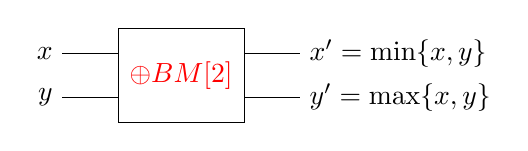
\begin{tikzpicture}[scale=0.7]
     % block
    \node[draw, rectangle, minimum width=1.6cm, minimum height=1.2cm] (blk) 
    {\color{red}$\oplus BM[2]$};
    
    % inputs
    \draw
    ($(blk.west)+(-1,0.4)$) node[left] {$x$}
    -- ($(blk.west)+(0,0.4)$);
    \draw
    ($(blk.west)+(-1,-0.4)$) node[left] {$y$}
    -- ($(blk.west)+(0,-0.4)$);
    
    % outputs, shifted up/down by 0.3 units
    \draw
    ($(blk.east)+(0,0.4)$) -- ($(blk.east)+(1,0.4)$)
    node[right] {$x'=\min\{x,y\}$};
    \draw
    ($(blk.east)+(0,-0.4)$) -- ($(blk.east)+(1,-0.4)$)
    node[right] {$y'=\max\{x,y\}$};
\end{tikzpicture}
    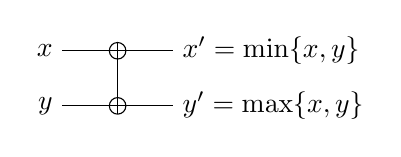
\begin{tikzpicture}[scale=0.7]
    % Draw horizontal lines for x and y
    \draw (-1,1) -- (1,1); % Line for x
    \draw (-1,0) -- (1,0); % Line for y
    
    % Draw vertical line connecting the comparator
    \draw (0,1.15) -- (0,-0.15);
    
    % Draw circles
    \draw (0,1) circle (0.15);
    \draw (0,0) circle (0.15);
    
    % Labels
    \node[left] at (-1,1) {$x$};
    \node[left] at (-1,0) {$y$};
    \node[right] at (1,1) {$x' = \min\{x, y\}$};
    \node[right] at (1,0) {$y' = \max\{x, y\}$};
\end{tikzpicture}
\end{center}

\begin{center}
    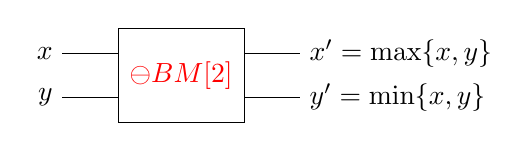
\begin{tikzpicture}[scale=0.7]
    % block
    \node[draw, rectangle, minimum width=1.6cm, minimum height=1.2cm] (blk) 
    {\color{red}$\ominus BM[2]$};
    
    % inputs
    \draw
    ($(blk.west)+(-1,0.4)$) node[left] {$x$}
    -- ($(blk.west)+(0,0.4)$);
    \draw
    ($(blk.west)+(-1,-0.4)$) node[left] {$y$}
    -- ($(blk.west)+(0,-0.4)$);
    
    % outputs, shifted up/down by 0.3 units
    \draw
    ($(blk.east)+(0,0.4)$) -- ($(blk.east)+(1,0.4)$)
    node[right] {$x'=\max\{x,y\}$};
    \draw
    ($(blk.east)+(0,-0.4)$) -- ($(blk.east)+(1,-0.4)$)
    node[right] {$y'=\min\{x,y\}$};
\end{tikzpicture}
    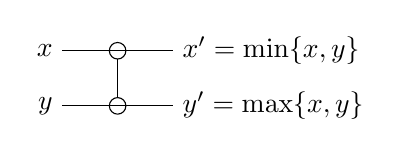
\begin{tikzpicture}[scale=0.7]
    % Draw horizontal lines for x and y
    \draw (-1,1) -- (1,1); % Line for x
    \draw (-1,0) -- (1,0); % Line for y
    
    % Draw vertical line connecting the comparator
    \draw (0,0.85) -- (0,0.15);
    
    % Draw circles
    \draw (0,1) circle (0.15);
    \draw (0,0) circle (0.15);
    
    % Labels
    \node[left] at (-1,1) {$x$};
    \node[left] at (-1,0) {$y$};
    \node[right] at (1,1) {$x' = \min\{x, y\}$};
    \node[right] at (1,0) {$y' = \max\{x, y\}$};
\end{tikzpicture}
\end{center}

Sulla destra una semplificazione in quanto reti con $n = 2$ sono dei comparatori.

Per una rete con $n$ fili, $\oplus BM [n]$, (quindi sequenza bitonica lunga $n$ in ingresso e ordinata in uscita), servono: 
\begin{itemize}
    \item $\log_2 n$ colonne
    \item $n/2$ comparatori per colonna
\end{itemize}

Ogni colonna ha comparatori a distanza pari a metà della colonna precedente (per $n=16$, prima colonna a distanza $8$, seconda a distanza $4$, \dots, fino a distanza 1 in $\log_2 n$ passi). Esempio per rete con $n = 16$:
\begin{center}
    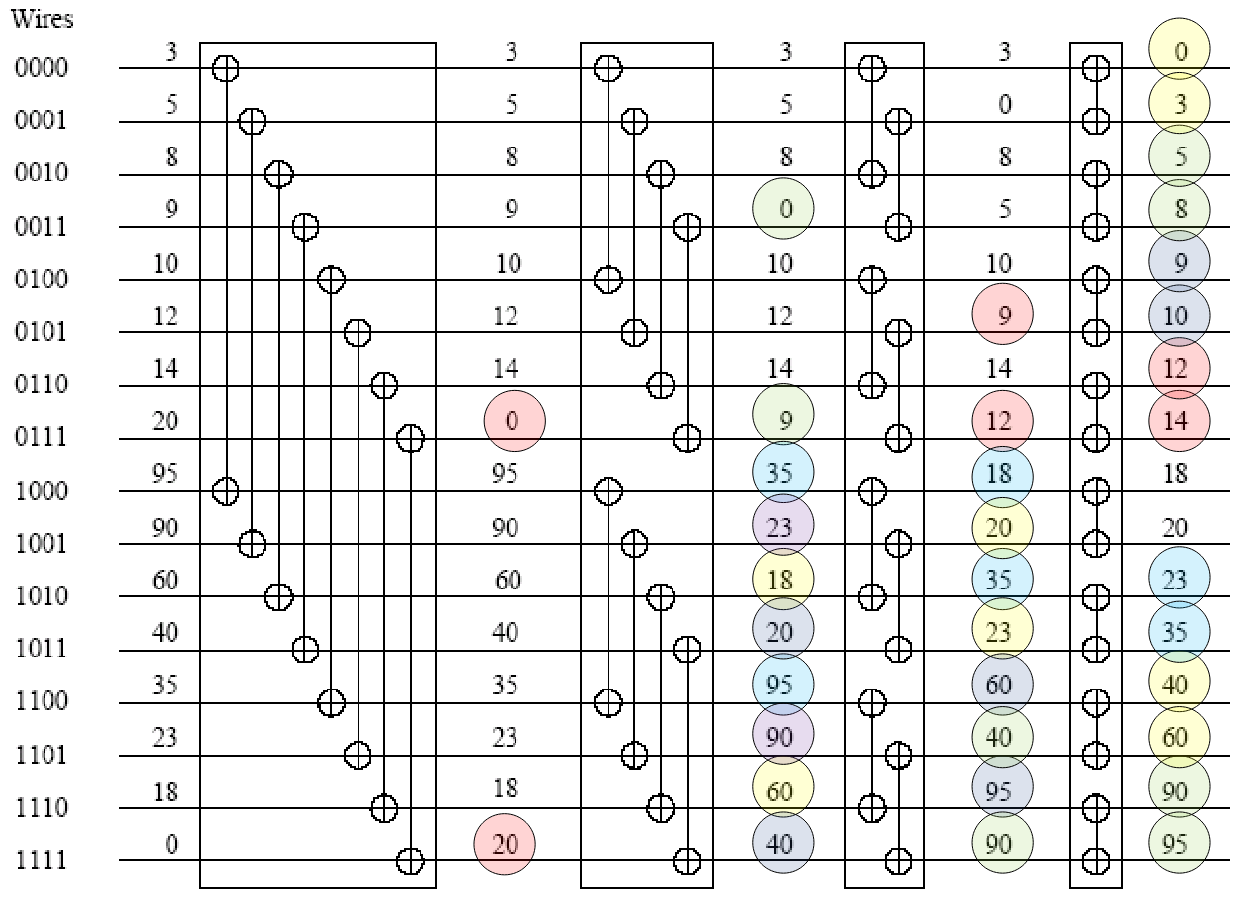
\includegraphics[width=0.79\columnwidth]{img/pattern/n16}
\end{center}

\paragraph{Costruzione di sequenza bitonica:} Con input una sequenza arbitraria, vogliamo ottenere una sequenza bitonica in output. Si può fare alternando i segni dei $BM$.

L'idea è quella di usare una rete con $(\log_2 n) - 1$ colonne: ogni $i$-esima colonna:
\begin{itemize}
    \item prende in input una sequenza bitonica di lunghezza $2^i$, a partire da $i=1$, una sequenza lunga 2 è banalmente bitonica
    
    \item si costruisce una sequenza bitonica lunga $2^{i+1}$ alternando $\oplus BM[2^i]$ con $\ominus BM[2^i]$, da fornire in input alla colonna successiva
\end{itemize}

L'ultima colonna avrà una $\oplus BM [n/2]$ e una $\ominus BM [n/2]$, per creare una sequenza bitonica lunga $n$.

\subsubsection{Ordinamento bitonico}

Si può ordinare una sequenza qualsiasi avendo: 
\begin{itemize}
    \item $(\log n) - 1$ step per costruire una sequenza bitonica a partire dall'input (come visto prima)
    
    \item aggiungere un comparatore $\oplus BM [n]$ alla fine per ordinare la sequenza
\end{itemize}

\paragraph{Complessità:} Per una sequenza lunga $n$, ogni step richiede: 
\begin{align*}
    T(n) & = T(n/2) + \log (n) \\
    & = \log (n) + \log (n/2) + \dots + 1 \\
    & = \sum_{i=0}^{\log n} i \\
    & = \frac{\log n \left((\log n) + 1\right)}{2} \\
    & = \Theta (\log^2 n) 
\end{align*}

%End L10

\end{document}

%Appunti notions: manca cap 9, da fare nelle ultime lezioni?